%%% The main file. It contains definitions of basic parameters and includes all other parts.

%% Settings for single-side (simplex) printing
% Margins: left 40mm, right 25mm, top and bottom 25mm
% (but beware, LaTeX adds 1in implicitly)
\documentclass[12pt,a4paper]{report}
\setlength\textwidth{145mm}
\setlength\textheight{247mm}
\setlength\oddsidemargin{15mm}
\setlength\evensidemargin{15mm}
\setlength\topmargin{0mm}
\setlength\headsep{0mm}
\setlength\headheight{0mm}
% \openright makes the following text appear on a right-hand page
\let\openright=\clearpage

%% Settings for two-sided (duplex) printing
% \documentclass[12pt,a4paper,twoside,openright]{report}
% \setlength\textwidth{145mm}
% \setlength\textheight{247mm}
% \setlength\oddsidemargin{14.2mm}
% \setlength\evensidemargin{0mm}
% \setlength\topmargin{0mm}
% \setlength\headsep{0mm}
% \setlength\headheight{0mm}
% \let\openright=\cleardoublepage

\usepackage[usenames]{xcolor} % typesetting in color
\usepackage{hyperref}         % pdf hyperlinks

%% Generate PDF/A-2u
\usepackage[a-2u]{pdfx}

%% Character encoding: usually latin2, cp1250 or utf8:
\usepackage[utf8]{inputenc}

%% Prefer Latin Modern fonts
\usepackage{lmodern}

%% Further useful packages (included in most LaTeX distributions)
\usepackage{amsmath}        % extensions for typesetting of math
\usepackage{amsfonts}       % math fonts
\usepackage{amsthm}         % theorems, definitions, etc.
\usepackage{bbding}         % various symbols (squares, asterisks, scissors, ...)
\usepackage{bm}             % boldface symbols (\bm)
\usepackage{graphicx}       % embedding of pictures
\usepackage{fancyvrb}       % improved verbatim environment
\usepackage{listings}       % code listings
\usepackage[numbers]{natbib}         % citation style AUTHOR (YEAR), or AUTHOR [NUMBER]
\usepackage[nottoc]{tocbibind} % makes sure that bibliography and the lists
			    % of figures/tables are included in the table
			    % of contents
\usepackage{dcolumn}        % improved alignment of table columns
\usepackage{booktabs}       % improved horizontal lines in tables
\usepackage{paralist}       % improved enumerate and itemize

\usepackage{inconsolata}
\usepackage[T1]{fontenc}

\usepackage[british]{babel}
\usepackage{caption}
\usepackage{subcaption}
\usepackage{changepage}

\usepackage{mystyle}

%%% Basic information on the thesis

% Thesis title in English (exactly as in the formal assignment)
\def\ThesisTitle{Framework and DSL for Ensemble-Based Access Control}

% Author of the thesis
\def\ThesisAuthor{Jan Matějek}

% Year when the thesis is submitted
\def\YearSubmitted{2019}

% Name of the department or institute, where the work was officially assigned
% (according to the Organizational Structure of MFF UK in English,
% or a full name of a department outside MFF)
\def\Department{Department of Distributed and Dependable Systems}

% Is it a department (katedra), or an institute (ústav)?
\def\DeptType{Department}

% Thesis supervisor: name, surname and titles
\def\Supervisor{doc. RNDr. Tomáš Bureš, Ph.D.}

% Supervisor's department (again according to Organizational structure of MFF)
\def\SupervisorsDepartment{Department of Distributed and Dependable Systems}

% Study programme and specialization
\def\StudyProgramme{Computer Science}
\def\StudyBranch{Software Systems}

% An optional dedication: you can thank whomever you wish (your supervisor,
% consultant, a person who lent the software, etc.)
\def\Dedication{%
I would like to thank my supervisor, doc. RNDr. Tomáš Bureš, Ph.D., for finding me an
interesting thesis topic on a relatively short notice, providing the source code of the
TCOOF-Trust prototype, and overall help with the work.

I would also like to thank my partners, Andy and Fronéma, for their support and
encouragement. Without them, I would probably never even start this work.
}

% Abstract (recommended length around 80-200 words; this is not a copy of your thesis assignment!)
\def\Abstract{%
Access control policies typically take the form of a set of static rules pertaining to
individual entities under control. This can be impractical in real-world scenarios:
authorization invariably depends on wider situational context which often tends to be
highly dynamic. This leads to increasingly complex rules, which have to change over time
to reflect the evolution of the controlled system.

Ensemble-based architectures allow dynamic formation of goal-oriented groups in systems
with large number of independent autonomous components. Because of the ad-hoc and
situation-aware nature of group formation, ensembles offer a novel way of approaching
access control.

The goal of this work is to design a Scala framework and internal DSL for describing
access control related situations via ensembles. In particular, the framework will
define ensemble semantics suitable for evaluating the ensembles and establishing access
control at runtime.
}

% 3 to 5 keywords (recommended), each enclosed in curly braces
\def\Keywords{%
{component ensembles}; {access control}; {domain-specific language}
}

%% The hyperref package for clickable links in PDF and also for storing
%% metadata to PDF (including the table of contents).
%% Most settings are pre-set by the pdfx package.
\hypersetup{unicode}
\hypersetup{breaklinks=true}

% Definitions of macros (see description inside)
\include{macros}

% Title page and various mandatory informational pages
\begin{document}
\include{title}

%%% A page with automatically generated table of contents of the master thesis

\tableofcontents

%%% Each chapter is kept in a separate file
\chapter{Introduction}

More and more areas of human activity are becoming computerized and connected to
ever-growing networks. This allows us to use these networks in novel, increasingly
powerful ways, as disparate systems are now able to communicate, aggregate knowledge,
and relay commands across domains. The growth and pervasiveness of Internet of Things
has a great promise for building cyber-physical networks, starting at smart homes,
smart buildings, and growing towards smart cities and large-scale smart grids.

At this scale, systems are necessarily heterogeneous. Devices from different
manufacturers are connected via custom communication protocols on virtual sub-networks
and managed by different organizations. Even if we limit the scope to a single
organization wanting to computerize its physical properties, different parts of the
system will usually be provided by different vendors, with separate connectivity and
separate management consoles.

To further complicate things, there is a strong demand for dynamic inter-connectivity.
Adding a new sensor to a smart home should be seamless, and allowing house guests to,
e.g., control music on the home stereo, should not be an insurmountable challenge. This
is even more important in smart cities, where almost by definition users cannot be known
in advance. And in enterprise environments, Bring-Your-Own-Device (BYOD) policies
require that employees are able to access company systems with their own smart devices.

Taken together, we are now surrounded by interconnected systems of enormous complexity.
Managing such systems is a significant challenge. Due to the nature of the requirements,
systems are also more vulnerable to malicious actors. And as their importance increases,
so does the value for an attacker. Therefore, security is of the utmost concern.

\bigskip

Our focus is on a particular aspect of system security, \textit{access control}, both in
physical and digital realms. Given a security policy, and the identities of users, it is
necessary to determine whether they are authorized to perform various actions. From the
physical realm, this usually means access to physical spaces, e.g., controlled by a
smart lock or a card reader; but also control of building infrastructure such as heating
and air conditioning, lights, etc. On the digital side, access permissions to data are
common. And in a highly dynamic system, it is necessary to determine whether one party
should be allowed to communicate with, and use services of, the counter-party.

Permissions are often context-dependent. In a smart city, users might only be allowed to
control resources that are near them, but denied access to more distant parts of the
grid. Autonomous cars coordinating on an intersection should allow communication between
each other, but only those that are actually engaged in the coordination task. Emergency
exits should remain locked most of the time, but allow anyone out when a fire alarm is
activated --- and emergency response teams should be authorized to access spaces that
have strong access controls under normal circumstances.

Current state-of-the-art access control systems are not well suited for these tasks. In
most approaches, a static set of rules is used for describing the security policy,
basically enumerating the situations that can arise and their resolutions. While modern
approaches such as Attribute-Based Access Control can take the situation context into
account, describing possibly overlapping situations causes an explosion of complexity.
The resulting policy is difficult to manage and audit, resulting in possible unintended
interactions between rules, or missed corner cases with undesired behavior.

This is especially true in heterogeneous, large-scale and highly dynamic systems. The
sheer number of agents and their possible interactions makes it difficult to enumerate
all combinations of circumstances and situations for the purpose of designing a
comprehensive security policy.

\bigskip

This work explores a different way of specifying security policies. We build on previous
research in the area of autonomic component ensembles, which provide a more natural way
of describing systems consisting of dynamic relationships between many independent
agents. Security situations are expressed in terms of ensembles, and the security policy
attaches rules to these ensembles.

Continuing the work from~\citep{isola2018}, our aim is to present a policy specification
language based on the ensemble model. We propose clear and well-defined semantics for
the language, allowing its user to specify ensembles and constraints for their existence
in a declarative way, with the goals of composability, readability and maintainability.

We also present an accompanying framework for identifying security situations and
resolving ensembles specified in the security policy. We make sure the system is capable
of observing and modeling non-computational entities and other agents that are not
controlled directly, such as humans. The framework can either respond to access control
queries directly, or emit a set of rules suitable for traditional systems.

%%%

\section{Structure of this Work}

We introduce a running example in chapter~\ref{running-example}. This is a scenario
which will serve as context and motivation for the rest of this work. In subsequent
chapters, we will refer back to the running example for showcases of certain features,
performance effects, etc.

In chapter~\ref{background} we look at problem background and related work in the
fields of ensemble based systems and dynamic access control. A brief overview of many
existing approaches is provided and evaluated with regard to our goals.

Chapter~\ref{overview} summarizes the problem, presents a broad overview of the proposed
solution, and restates our requirements in concrete terms.

Chapter~\ref{dsl} is intended as a user guide to the TCOOF-Trust framework and language.
It contains explanations of core concepts and their semantics, provides practical
examples and a full reference of the features of the DSL. It also contains a full
implementation of the security policy of the running example.

Translation process from the DSL to a constraint satisfaction problem is described in
chapter~\ref{impl}, together with implementation details for the DSL constructs.

In chapter~\ref{evaluation} we evaluate performance of the basic operations of the
framework, and then test the running example implementation in a number of synthetic and
real-world-like scenarios.

Finally, chapter~\ref{conclusion} summarizes our findings and concludes the work.


\chapter{Running Example}
\label{running-example}

For our running example, we use a modified scenario based on a real-life problem, which
was first introduced in \citep{isola2018}. We will refer back to this scenario
throughout the work, in order to showcase problems, features of the DSL, and
implementation details.

\section{Scenario}

The scenario models a company that works on sensitive projects for its clients. At any
given time, multiple projects can be developed in parallel. Developers working on the
same project must be able to cooperate. However, to limit exposure of sensitive
intellectual property, developers from different projects should not come into contact
with each other; namely, developers of two different projects are not allowed to stay in
the same room while in the company building. To this end, each developer has a smart
device (mobile phone, smart watch, etc.) that can direct them to the appropriate rooms.

We assume that each developer is assigned to exactly one project. Only two types of
rooms are considered: workrooms and lunchrooms.

Workrooms are open whenever the building is open, which is from 7:30~AM to 9~PM. Each
workroom is assigned to a particular project. All developers on a project are permitted
to enter all workrooms for that project, to allow for efficient collaboration. We assume
that workroom assignment is fixed for the duration of our scenario and that it provides
enough capacity for all developers of a given project.

Lunchrooms only open around midday, from 11:30~AM to 3~PM. Each lunchroom has a set
maximum occupancy. We expect that there will not be enough lunchrooms to seat all
developers, esp. with the constraint that developers from different projects must not
meet in the same room. Therefore, room assignment must be dynamic. Developers will be
equipped with smart devices which can send seating requests and display the current
situation.

\medskip

Our interest lies in access permissions. Specifically, we want to investigate which
developers can enter which rooms at various times and under various conditions, and how
an access control system could handle a given situation.

\begin{figure}[t]
    \centering
    \includegraphics[width=1\linewidth]{img/lunch-rules.pdf}
    \caption{Example scenario with workrooms and lunchrooms}
    \label{fig:lunch-rules}
\end{figure}

Figure~\ref{fig:lunch-rules} illustrates a possible situation. Developers on blue and
red projects are moving around in the building, which has three lunchrooms and three
workrooms. Two workrooms (computer symbol) are assigned to the red project and one is
assigned to the blue project, as indicated by the symbol color. Lunchrooms (food symbol)
are not assigned to projects. Each room has a capacity of four people.

There is a red, blue or black lock on each door. Red and blue indicates that the door is
open to developers of the corresponding project. Black indicates that anyone can open
the door. The lock on room D is closed, showing that nobody can enter. In this case, it
is because the room is full.

Room B is also full, but the lock remains open, because our security policy does not
take workroom capacity into account.

The red worker in the middle is allowed to enter room A, because it is a workroom
assigned to a red project. The hungry red worker is not allowed to enter room D,
however, because the room is full. She would be allowed to enter room E, currently open
to developers of red project, but the hungry blue worker in the middle cannot do that.
There is already a red worker inside, and the security policy disallows developers from
different projects to meet in the same room. Hungry blue worker at the bottom can enter
room F, because it is empty, so no security conflict arises.

\section{Workroom Assignment}

If we ignore lunchrooms for a moment, the problem is relatively simple. Access
permissions are known in advance. At night, no rooms are open and nobody is allowed to
enter. In the day, every developer assigned to a particular project is allowed to enter
every workroom assigned to that same project. We can enumerate the available workrooms,
and for each one, enumerate all persons allowed to enter that room. Only those people
are allowed to enter, and no other access permissions exist. The rules are fixed and
don't need to be updated except when scenario definition changes.

\begin{figure}[ht]
    \centering
    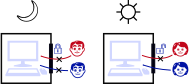
\includegraphics[width=1\linewidth]{img/workroom-access.pdf}
    \caption{Workrooms at night and in the day}
    \label{fig:workroom-access}
\end{figure}

Figure~\ref{fig:workroom-access} shows all possible configurations. Either it is night
time, in which case nobody can enter, or it is daytime, and blue developers can enter,
while red ones cannot. This scenario is easy to solve even in traditional entity-based
access control systems. The only dynamic parameter is time of day, which is commonly
supported on contemporary electronic locks.

\section{Lunchroom Assignment}

During lunch hours, a developer can request seating in a lunchroom. This introduces a
dynamic and unpredictable element. It is no longer sufficient to \textit{enforce} access
control rules, we need to re-evaluate the situation and generate new access grants.

\medskip

There are several possible approaches to this situation. One option is to leave the
choice to the human: during lunch hours, every developer is allowed to enter every
lunchroom, except when (a) the lunchroom is full, or (b) developers from a different
project are already present in the lunchroom. The advantage of this approach is twofold.
First of all, it gives greater freedom to the developers. The system is not trying to
make decisions for them, and everyone can choose a lunchroom based on their own
criteria, such as how close it is, where their friends sit, etc. Second, because the
system does not need to make choices, it is computationally simpler. We need to monitor
the situation and update access grants based on current seating and room capacity, but
we can still describe the situation using conditional entity-based rules.

There are some drawbacks, too. When individual developers choose lunchrooms for
themselves, they only take their local context into account. This can lead to a
situation shown on figure~\ref{fig:lunch-inefficient}. Red developers have occupied
all the available lunchrooms. Even though there is more than enough total available
seats, none of the hungry blue developers can use them.

There is also no way to reserve a seat in advance; a developer could head out towards
their favorite lunchroom, only to find out that it is occupied and they need to go
elsewhere.

\begin{figure}[ht]
    \centering
    \includegraphics[width=0.67\linewidth]{img/lunch-inefficient.pdf}
    \caption{Inefficient use of available lunchrooms}
    \label{fig:lunch-inefficient}
\end{figure}

\medskip

On the opposite end of the spectrum, we can have the access control system make all the
decisions. We are working with the assumption that developers are free to choose
\textit{when} they want lunch, so we cannot simply pre-generate fixed time slots and
seats and solve a scheduling problem. However, we can still assign a particular
lunchroom whenever a developer requests a seat. The rule would be as follows: during
lunch hours, a developer can request a lunchroom. When a valid seat becomes available,
the developer is allowed to enter the assigned lunchroom once. When they leave the
lunchroom, their seat is freed for next requests.

This is the variant that we will be using in the rest of this work. It gives us the
opportunity to explore behavior of an access control system with regards to solving
conflicting and/or overlapping requirements.

\medskip

We must note, however, that in the real world, a less strict system would be preferable.
Perhaps a hybrid of the two outlined here: allow the developers to choose a lunchroom
based on individual preferences, reserve a seat through a smart device, while employing
heuristics to keep some free lunchrooms so that no project is starved, both in the
technical and the literal sense.

\section{Assignment Criteria}

When assigning lunchrooms, we must satisfy the scenario rules: developers from
different project must not be allowed to enter the same room, and we cannot assign
more developers to a lunchroom than its capacity. But in addition, we might want to
optimize for other criteria.

First of all, we want to achieve good utilization and availability of lunchrooms. More
specifically, every lunch request should be serviced as soon as possible, and thus every
developer should be able to have lunch at the time of their choosing. This means two
things: (1) we need to seat as many developers as possible at the same time, and (2) at
any given time, we should be able to seat a developer from any project.

While obviously limited by total capacity, there is a lot of room for different choices
with regard to these criteria. Consider a situation where a group of 6 developers from
project $A$ and a group of 4 developers from project $B$ request lunch simultaneously,
and there is only one free lunchroom available. By (1), we should seat the group from
project $A$, because it is bigger. But if all the other lunchrooms are occupied by
project $A$, we should probably give the room to the $B$ group to better achieve (2) ---
this would reserve the free space for more developers of project $B$, while we can
expect spaces for $A$ developers to become available in the other lunchrooms.

\medskip

We could continue adding criteria, of course. Earlier requests should have priority. It
might be desirable to assign lunchrooms that are physically close to the requester. We
might try to keep groups together. Perhaps requests should be prioritized by employee
seniority, or maybe we should even keep reserved seats for the bosses at all times. Each
developer could sort the lunchrooms by preference and their selection should be taken
into account.

Obviously, each additional criterion is making the problem more complex. It is not our
goal to solve this complexity; the point here is to show that requirements can vary and
this needs to be taken into consideration.

\chapter{Background and Related Work}
\label{background}

\section{Ensemble-Based Architectures}
\label{background:ensembles}

The complexity of managing a system grows with its size. This has traditionally been
handled through hierarchical decomposition, component-oriented programming, and similar
techniques. With the rise of the Internet of Things, however, we are reaching the limits
of these approaches. If the environment consists of many independent agents with no
clear functional hierarchy, it is impractical to impose a top-down view of control.
There is no single point of access to a ``swarm'' of sensors, smart things, and
cyber-physical systems in general, especially when these are distributed over a large
area with no promise of reliable connectivity and continued availability. The use-cases
are new, too: clients want to access the system from different locations and
perspectives, use different services in different configurations, and take advantage of
the inherent dynamicity.

The problem is partially solved through \textit{Service-Oriented Architectures}
\citep{SOA}. SOA revolves around modular, dynamically discovered and dynamically bound
services. Unlike a typical ``hard-coded'' component-based system, SOA can deal with
small services that are randomly appearing and disappearing from the network. There are
limitations, though. SOA is still a top-down approach that assumes its parts are
discrete services. This is not necessarily true with IoT. Consider a home sensor
network. SOA can expose every sensor as its own service, but then it falls to the client
to locate, e.g., all sensors in a single room. Alternately, the whole network could be a
single service, but then it needs to have ``zoom in on a single room'' as a feature.
This gets complicated when the query changes, e.g., when locating all temperature
sensors. The issue is more pronounced when considering a heterogeneous city-wide network
of smart things. Also, service discovery starts being a difficult problem when the
number of services grows to tens of thousands.

A whole other issue is agent collaboration. Certain problems lend themselves to
distributed approaches --- e.g., self-driving cars collaborating to find parking spaces
along their driving routes. While it is possible to create a centralized service for
this task, it would be more practical to have the agents collaborate directly and
locally. This is not a problem that SOA can solve, and indeed it is unsuitable for any
kind of top-down approach. Instead, we need to look towards multi-agent systems to
manage the collaboration, and possibly some other approaches that will allow the agents
to locate each other, establish communication links, organize and reorganize.

To restate: we are experiencing an explosion of the size of cyber-physical systems and
the number of independent computing devices, and traditional approaches fail to use
these systems efficiently. There is a growing need to organize highly dynamic systems
that consist of many independent agents. Not only is a different approach required, we
actually need different abstractions.

\medskip

One such abstraction is the \textit{ensemble}. An ensemble is a loose coalition of
\textit{components} formed around a shared goal. A component can be any kind of moving
part: in a software system, a component would be a module, object, service, any piece of
code performing a particular functionality. In the world of cyber-physical systems, a
component can be a computer, an IoT device, a drone, etc. As we show in this work, we
can even model humans, rooms and other non-computational entities as components.

Members of an ensemble inhabit specific \textit{roles}, which are usually described in
terms of capabilities or services a component can provide. This decouples concrete
components from the ensemble. For example, an ensemble providing environmental data for
a HVAC\footnote{Heating, Ventilation, Air Conditioning} system could have a
``thermometer'' role, a ``CO\textsubscript{2} detector'' role, and an ``uplink'' role
which handles Internet connectivity. These would be inhabited by appropriate devices,
without regard to which specific device is providing which service.

A single component can perform multiple roles in the same ensemble (e.g., an
Internet-capable thermometer can function both as a sensor and as an uplink), or be a
member of several different ensembles (the same uplink can serve multiple sensor suites
at the same time). It is also conceptually simple to replace a component with a
different one in the same role, in case the former member becomes unavailable or no
longer fits the ensemble's parameters.

Ensembles are composable; an ensemble can contain any number of sub-ensembles, which in
turn can be composed of more sub-ensembles. Sometimes it is useful to set up a role
which can be inhabited by a sub-ensemble.

\medskip

One of the key features of an ensemble-based architecture is its high level of
dynamicity. Ensembles are formed and dissolved when needed. Similarly, membership in an
ensemble is driven by current context and conditions, not by any sort of explicit
registration. Therefore, the natural way to specify ensembles is declarative. We can use
predicates over component properties and the local conditions. E.g., a smart parking lot
can define an ensemble as ``parking meter, plus all vehicles seeking parking within 10
minutes from it.''

This meshes well with ideas of autonomic computing~\citep{IBM2003}: individual components
could be able to determine ensemble membership based on their own knowledge, without a
central coordinator. Alternately, when a global perspective is available, a coordinator
can use all available information to optimize ensemble membership and role assignment,
and can be flexible in responding to change.

Due to its ephemeral nature, it is difficult to work with an ensemble ``from the
outside''. In an autonomic system, ensembles might not even be visible from the outside,
their existence known only to the individual members. And even with a central
coordinator, there are some challenges: for example, an ensemble can dissolve at any
time and its constituent components can be reassigned. There is no way to maintain a
persistent reference to a particular ensemble or a role within it. Instead, the ensemble
system should be considered self-organizing and self-governing. A user of the ensemble
system can post goals, and the system will ensure that ensembles are formed to resolve
that goal.

\subsection{Related Work}

Ensembles present a perspective which differs significantly from traditional views of
component systems. For this reason, new methodologies and paradigms are being designed
for efficient programming of ensemble systems.

\medskip

\textit{Software Component Ensemble Language} was introduced in \citep{SCEL2013} in 2013
and refined a year later in \citep{SCEL2014}. SCEL is designed as a ``kernel'' language,
a mostly abstract grammar that is supposed to be a building block for more concrete and
full-featured languages. Its paradigm is built on four concepts: \textit{knowledge} of
individual components; \textit{behaviors} operating over knowledge bases;
\textit{aggregations} as collections of components; and finally \textit{policies} that
can control and adapt execution of behaviors. Each component is represented as an
interface exposing its knowledge base, available behaviors, and governing policies.

Despite having ``ensemble'' in the name, there is no explicit notion of an ensemble nor
a role. They exist implicitly, via the ability to control targets of actions with
logical predicates.

Interestingly, the SCEL paper~\citep{SCEL2014} shows an access control sub-language as
an example of the policy concept. However, the language is used to protect processes on
the level of one component, and its capability to consider broader situation context is
limited, so it is of little interest to the topic of this work.

\medskip

HELENA, from \textit{Handling massively distributed systems with ELaborate ENsemble
Architectures} \citep{HELENA2014} \citep{HELENA2016}, is a rigorous formal approach to
ensemble-based systems, focused primarily on the role concept. The goal of the design is
to enable formal verification of ensemble behavior. Role operations are specified by
a~labeled transition system, and ensembles are modeled as automata. Components are
considered resources for the roles they can fulfill, but are themselves passive; any
active behavior is initiated through the role abstraction.

As the HELENA approach examines the problem from the role level, the process of forming
an ensemble is left unexplored. Finding components to inhabit roles is assumed to be
implicit.

\medskip

The \textit{Distributed Emergent Ensembles of Components} (DEECo) model
\citep{DEECo2016} is a more practice-oriented approach, tailored for use in IoT
applications. It defines a paradigm of \textit{ensemble-based component systems}, where
components, roles, and ensembles are all first-class objects. The DEECo paper also
discusses the question of reliability of communication and presumes use of mesh
networking.

Membership in an ensemble is determined by a \textit{membership condition} over
components' knowledge attributes. Component roles are modeled as interfaces, prescribing
the knowledge attributes that must be available to the ensemble. Ensemble definition
further specifies what knowledge is exchanged between members, when, and how often.

Ensemble formation is initiated by a \textit{coordinator}. Each ensemble specifies a
single coordinator role. The component which inhabits that role will look for other
members via local or routed broadcast on the network, and facilitate the knowledge
exchange processes. While the paper doesn't elaborate on this, the concept is
nevertheless important, as it basically imposes locality on the search for members.

\medskip

A follow-up paper~\citep{dynamic2017} expands on the idea of search locality, adds
discussion of performance issues, and introduces the concept of filtering as a way to
limit the number of components in consideration. It also adds a concept of
\textit{fitness}, a quality score of the formed ensemble. For example, it is possible to
specify that an ensemble consisting of nearby components is a better candidate than an
ensemble whose components are far from each other.

In~\citep{tcoof2017} an architecture definition language called \textit{Trait-based
Coalition Formation ADL} (TCOF-ADL) is presented. Its express goal is to facilitate
selection of components and formation of ensembles, while ensuring that formation
responsibilities are properly distributed between agents in the ensemble system. It
provides some basic predicates and allows components to be extended with ensemble
formation related traits such as location awareness, data prediction, and a statistical
evaluator. The language is implemented as a Scala-internal DSL and employs a constraint
solver to help with ensemble membership resolution.

A variant of TCOF-ADL, named TCOOF-Trust\footnote{The additional ``O'' in the name is
not explained. Presumably it comes from changing ``coalition'' to ``coordination'' in
the acronym.}, is presented in~\citep{isola2018}. The paper specifically deals with
application of ensemble concepts to access control, and this work is a direct follow-up
to the same research. The TCOOF-Trust language reuses some of the original constructs,
as well as the ensemble formation engine, and adds commands related to access control
decisions.

\section{Access Control in Dynamic Systems}
\label{background:access}

Historically, access control tended to be rule-based and local to specific resources,
such as files or concrete objects. In UNIX, for example, each file has an owner and a
group, and a fixed bitmap of permissions that can be granted or denied to the owner,
members of the group, or everyone else. An improvement to this system is an
\textit{Access Control List} (ACL) attached to an object, which can list an arbitrary
number of users, groups, and their permissions.

As system complexity grows, this is no longer a sufficient solution. Many contemporary
systems use some variant of \textit{Role-Based Access Control}~\citep{rbac1995} (RBAC).
Access control rules are expressed as tuples: (\textit{role}, \textit{operation},
\textit{subject}), authorizing members of \textit{role} to perform \textit{operation} on
a \textit{subject} resource. In addition, roles can be arranged in a hierarchy, so that
a role higher in the hierarchy inherits all permissions of lower roles. This naturally
fits human organizational hierarchies: e.g., a supervisor role will usually inherit all
permissions of the worker role, without need to specify them again.

A single user can be assigned to any number of roles. This provides an important
abstraction and simplifies user management, as it is now possible to grant or revoke
user privileges simply by modifying their role assignment. A more recent
\textit{Organization-based Access Control}~\citep{orbac2003} (OrBAC) model adds another
layer of abstraction: each of \textit{role}, \textit{operation} and \textit{subject}s in
the master policy can now be ``implemented'' by a corresponding object in a local
environment. This enables sharing policies between organizations at design-time and
collaboration at run-time, as two organizations can cross-authorize their users in
compatible roles.

As described, RBAC-like policies are not aware of wider context. Role $R$ has permission
to perform operation $O$ on subject $S$ at all times, regardless of situation or current
conditions. That is not good enough for many real-world scenarios, where context plays
an important role. For instance, a ``worker'' should have permission to ``enter'' the
``workspace'' --- but only during work hours.

Several approaches arose to close this gap. \textit{Context-Sensitive
RBAC}~\citep{contextkumar2002} adds context information to roles, operations, and
subjects, and attaches predicates over the contexts to individual access control rules.
Similarly, \textit{Context-Aware RBAC}~\citep{contextkulkarni2008} introduces
preconditions that can query context information before allowing the rule to apply. In
addition, a ``context guard'' predicate can be specified, which must hold true in order
for active sessions to remain open. In~\citep{contextrbac2004}, context constraints are
separated into those that can be evaluated at design-time and those that must be
evaluated at run-time, and a development methodology for constrained rules is presented.

In recent years, \textit{Attribute-based Access Control}~\citep{abac2014} (ABAC) is
gaining popularity because of its even greater flexibility. In ABAC, permissions are not
attached to roles, but to arbitrary expressions over attributes of users and subjects.
As an example, RBAC could be considered a special case of ABAC, with the only attribute
under consideration being the list of user's roles. But every object can have any number
of attributes and these can dynamically reflect current situation. Attributes of
environment, such as current date and time, can also be accessed.

A popular realization of the ABAC model is OASIS XACML~\citep{xacml2013} standard, which
is an XML-based policy language, and a more developer-friendly language
ALFA~\citep{alfa} that translates directly to XACML. Developers can describe rules using
a large number of built-in predicates, or they can define custom functions for more
complex situations.

\medskip

The main limitation of these approaches, which we will collectively call ``rule-based'',
is the actor-action-subject perspective. ABAC is capable of querying the situation, but
the query still originates from a static description of applicable actors, actions, and
subjects. In other words, rules can query context, but context cannot influence rules.

This makes rule-based approaches highly impractical in scenarios where the context does
in fact cause the rules to change. The implementation of such context-dependent security
policy is scattered across many different rules, which makes it hard to audit, maintain
and debug. In fact, it is difficult to enumerate the rules that should be affected in
the first place.

One example is dynamic global state which cross-cuts ordinary rules. For instance, a
``night policy'' might be different from a ``day policy''. Affected rules would need to
have two variants, and updating one of the policies couldn't be done in one place. In
addition, if global states can overlap (consider a ``lock-down state'' when every door
only opens for members of a designated responder group and nobody else), complexity can
grow exponentially. This growth manifests in every affected rule, possibly to the point
where it is more practical to go outside the ABAC system and simply maintain separate
manually deployed policy configurations.

In highly dynamic systems, such as IoT networks, the same limitation can be seen from a
different angle: it is burdensome to express every possible combination of actors,
actions, and subjects beforehand. Dynamic relationships arise, form, and dissolve
throughout the life of the system. In our running example, a person is not allowed to
enter a room if another person working on a different project is already inside that
room. Such rule can be expressed as a context query with some creative use of
attributes, but it is more natural to query the context first and dynamically form the
rule afterwards.

\medskip

A number of so-called ``adaptive security'' solutions and frameworks have been proposed
to get around this limitation, each with their own pros and cons.

dynSMAUG~\citep{dynsmaug2017} paper works with the concept of a \textit{situation}
distinct from \textit{context}. While context is a collection of information on the
actors and the environment at a specific point in time, a situation is a time frame ---
an interval in which some context predicates hold true, possibly including particular
sequences of events. Situations are defined separately from the security policy in a
SQL-like language Esper~\citep{esper}, and currently applicable situations are exposed
as attributes queryable by XACML/ALFA languages.

While the model is sound, the need to describe the policy in two phases and in two
different languages is impractical in terms of maintainability. Furthermore, the Esper
language is powerful but also very complex even for simple cases.

A self-learning model was presented in \citep{adaptivesec-bashar2012}. Protected assets,
operational goals and possible threats are modeled and then compiled to a fuzzy decision
network. This network can evaluate the state of the system at run-time and configure or
reconfigure applicable security policies. This solution, however, is limited to
reasoning about a closed system, with no consideration for independent agents.

The solution presented in \citep{saleemi_framework_2011} uses inference rules based on
logic programming to build higher-level context information from lower-level knowledge
(such as sensor readings). Resulting high-level knowledge is then used as a basis for
security actions. This enables the policy designer to make security decisions at the
appropriate level of abstraction.

\chapter{Solution Overview}
\label{overview}

Contemporary access control models are overwhelmingly of the rule-based variety --- that
is, the policy is a set of rules in the format ``\textit{actor} is permitted to
\textit{action} on \textit{subject}''. They do not cope well with highly dynamic
systems, where strong situational awareness and ability to handle ad-hoc formed
relationships between independent agents is required. Adaptive models have been
proposed, which can handle some parts of the problem, but there is currently no
consensus on the appropriate way to control systems like smart spaces, IoT sensor
swarms, and other large-scale dynamic environments.

We are interested in a model that would have all of the following properties:

\begin{itemize}
\item \textit{Situational awareness.} The system should be context-aware by default,
able to detect situations based on low-level information, and make situation-appropriate
decisions.

\item \textit{Dynamicity.} The system should cope well with environments consisting of a
large number of agents that can appear, disappear, and form ad-hoc relationships at any
time. It should enable decomposition of the environment into logical groups, and update
immediately when availability or properties of the group members change.

\item \textit{Composability.} It should be possible to break the policy down to
functional parts and build higher levels of policy from the lower-level components.

It should also be possible to develop parts of the security policy separately, even if
they relate to the same actors or subjects. The resulting policies should be applicable
at the same time if their end results do not conflict, and there should be a way to
resolve conflicts that arise.

\item \textit{Maintainability.} The policy specification should enable good engineering
practices. Related concepts should be specified close together. Security decisions
should be made at the appropriate abstraction level. It should be easy to see which
parts of the policy are affected by a change, or which parts must be changed to achieve
the desired effect.
\end{itemize}

The idea explored in this work is to describe security situations in terms of ensembles
with attached access control decisions, have a solver element identify which components
are members of which ensembles, and apply the rules on them.

Ensemble-based architectures naturally possess the first three desired properties. They
are designed for large-scale systems composed of many independent agents, and are
suitable for highly dynamic environments. Ensemble formation depends on current context.
An ensemble is a logical group of components, so it is a decomposition of the larger
system. It can also itself be constructed from sub-ensembles, allowing composability.
Components are not limited to a single ensemble, so ensembles can overlap.

As for the fourth property, maintainability, that depends for the most part on the
design of a specification language and choice of the right abstractions. As explained in
section~\ref{background:ensembles}, declarative specification is a natural approach for
ensembles. Another notable feature we are interested in is composability on the language
level, not just on the conceptual level. Work on SCEL and DEECo is a~good inspiration
here.

\medskip

To make ensemble-based architectures applicable to the problem of dynamic access
control, we will need to tweak some of their properties.

First of all, ensemble-based systems are usually distributed and components
self-organize based on their knowledge. That approach is obviously not applicable to
access control. We will require a trusted supervisor with complete information to form
the ensembles and enforce the rules.

Another issue is beyond-control entities. Access control systems routinely deal with
independent agents beyond their control, such as humans; after all, the whole point of
an access control system is to make decisions that limit actions of beyond-control
agents. Ensemble systems, on the other hand, tend to require agent cooperation in order
to achieve their goals.

The ensembles that we use are not goal-oriented, however. There is no reason to control
actions of individual components or direct them imperatively. From the access control
point of view, component knowledge --- and indeed the ensemble structure as such --- is
purely descriptive. We can represent beyond-control entities as virtual components and
gather knowledge about them indirectly via sensors. E.g., the system can track a human's
position with an indoor positioning system and their smartphone, and can monitor room
capacity by counting incoming and outgoing door openings.

Using a central supervisor happens to help us here, too. It is a good place to store
the collected knowledge, and to perform computations that would be done on the
components in a more traditional ensemble system.

\section{Practical Example}

\begin{figure}[ht]
    \centering
    \includegraphics[width=0.68\linewidth]{img/ensemble-norequest.pdf}
    \caption{Example situation: no outstanding lunch requests}
    \label{fig:norequests}
\end{figure}

Figure~\ref{fig:norequests} illustrates a part of our running example. There are two
lunchrooms, each with six available spaces. Two people from a blue project are already
eating in the left one, and three people from a red project are eating in the right one.
The translucent shapes indicate two existing ensembles, each of which is formed around a
door lock. Membership in an ensemble grants the person a permission to open the
corresponding lock.

In the first picture, nobody is requesting access to a lunchroom. The only people
allowed to unlock the doors are those already inside, who should obviously be allowed to
leave.

\begin{figure}[h]
    \centering
    \includegraphics[width=0.68\linewidth]{img/ensemble-withrequest.pdf}
    \caption{Example situation: new lunch requests}
    \label{fig:withrequests}
\end{figure}

In picture~\ref{fig:withrequests}, four more people from the red project are hungry, as
indicated by thought bubbles. When the system is informed of this, it should allocate
lunchroom seats to the hungry people. The red ensemble extends to include three of the
hungry people --- but not the fourth, because there is no more space for them in the
lunchroom. The blue ensemble doesn't include them, because they are working on a red
project, and this would violate the constraint that people from different projects
cannot eat together.

\medskip

The example in figure~\ref{lst:pseudo} uses a pseudo-language to concisely express the
ensemble configuration, which roles exist, and what constraints limit the available
solutions. The \lstinline{allow} verbs also specify access control rules to apply on the
ensemble.

\begin{figure}[b]
    \begin{lstlisting}[style=pseudo]
ensemble Lunchroom {
    role Room = select 1 of all rooms
    role Eaters = select all of Room inhabitants
    role Requesters = select some of all hungry

    constraint {(Eaters + Requesters) must not exceed Room capacity}
    constraint {all Eaters and Requesters must have the same project}

    allow Requesters to enter Room
    allow Eaters to leave Room
}

constraint {Room from every Lunchroom must be distinct}
constraint {Requesters from every Lunchroom must be disjoint}
\end{lstlisting}
    \caption{Pseudo-code for specifying a small ensemble configuration}
    \label{lst:pseudo}
\end{figure}

The code defines an ensemble type for a single lunchroom. Three roles are defined:
\lstinline{Room} is the selected lunchroom, \lstinline{Eaters} are people already
inside, and \lstinline{Requesters} are those who are waiting for a seat. All eaters are
selected, but only some requesters. This prevents a requester from displacing someone
who is already in the room. The ensemble-local constraints ensure that we do not pick
more people than we can (which effectively only limits the number of new picks) and that
all selected people are from the same project.

Global constraints, applied over all instances of \lstinline{Lunchroom}, ensure that no
more than one ensemble is formed per room and that a single requester is not picked for
more than one lunchroom. It is important to note that ensembles are generally allowed to
overlap; without this constraint, situation on picture~\ref{fig:overlap} would be
perfectly valid. The same requester would take up space in both lunchrooms, pushing out
the hungry person in the top left.

\begin{figure}[h]
    \centering
    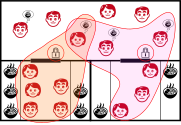
\includegraphics[width=0.68\linewidth]{img/ensemble-overlap.pdf}
    \caption{Example situation: same person is selected for both rooms}
    \label{fig:overlap}
\end{figure}

Given a definition similar to the example above, the supervisor should analyze the
current situation, choose an appropriate assignment of components to roles, and grant
the specified permissions.

\section{Goals Revisited}

There are now several open problems that must be solved in order to make the above
example actually work. There are also several more necessary features that are not shown
in the example. We can divide the goals into two distinct areas: the specification
language, and an implementation of the supervisor element. In the rest of the text, we
will call this supervisor element the \textit{solver}.

\subsection{Specification Language}

Our example uses pseudo-code to outline the desired semantics. We need a language that
is parsable by the solver and expressive enough to support all the desired features. Our
goal is to design such language and specify its semantics in detail.

Language design poses a problem on its own. It would be ideal to reuse an existing
language and only extend it to support our use-case. For this reason, we decided to
implement an internal domain-specific language (DSL). Scala~\citep{scala} was chosen as
the host language for its flexible syntax and strong typing system. Scala gives us a
repertoire of powerful language features, operators, and primitives readily available
for the DSL. We are thus free to concentrate on the specification semantics.

At its most basic, our language must allow definition of ensembles, roles within them,
and membership predicates for role inhabitants. As shown in the example, it must also be
possible to specify arbitrary constraints, applicable both locally within the ensemble
and globally over multiple ensembles. 

Next, the language must provide a way to specify when an ensemble is applicable. In our
running example, lunchrooms should only open during lunch hours. This is partially
possible with arbitrary constraints on the ensemble formation: if one of the constraints
is ``it must be lunch time'', the ensemble will simply not form at other times. However,
an ability to \textit{enforce} that a particular ensemble is formed might be useful in
certain use cases.

Many ensemble configurations can have multiple solutions. Looking back at
picture~\ref{fig:withrequests}, there is nothing in the pseudo-code specification
telling the red ensemble to find as many hungry people as it can. If the ensemble
remained the same as on picture~\ref{fig:norequests}, it would still fit all the
constraints. The specification language should thus have a way of indicating ``solution
quality'', or scoring a~given solution.

Finally, as we are interested in access control, it must be possible to attach security
decisions to the ensembles and specify when and how they apply. A~reasonable format is
RBAC-like \textit{actor-action-subject} --- it is familiar, and at the point when the
rule is applied, we have already expressed all contextual awareness by forming the
ensemble.

\subsection{Solver Implementation}

The second goal is to have a working implementation of the supervisor element. It should
process a policy specification and determine which ensembles are applicable and which
components will inhabit which roles. When the specification is ambiguous, the solver
should choose a solution that satisfies all constraints.

Given a set of components and arbitrary constraints, finding a valid role assignment can
be transformed into a constraint satisfaction problem. This would allow us to reuse an
existing constraint solver library instead of creating our own. Therefore, the solver
should be capable of converting the relevant parts of policy description into a
representation appropriate for a constraint solver.

As previously stated, some scenarios can have a method of scoring the solution quality.
The solver must be able to configure itself to either find any viable solution, or to
find a solution optimal in some variable. Furthermore, certain problems can be described
in multiple different ways, and different descriptions can have different performance
characteristics. The solver must be amenable to such tweaks, possibly even configurable
in how it explores the solution space.

And of course, after a solution is found, the solver must allow users to inspect the
solution and execute access control queries.

\subsection{Solution Novelty}

This work is a direct follow-up to the paper~\citep{isola2018}, which introduced both
the idea of using ensembles for access control, and the Scala DSL implementation which
is the basis for our framework. That implementation was presented as a proof of concept,
mainly intended for rapid prototyping. Our aim is to improve upon it in several notable
areas.

On the DSL side, our main goal is to extend, refine, and stabilize the set of available
language constructs. Each function, method, or construct should have well-defined
semantics and a~clearly stated purpose.

Another goal is to ensure that using the DSL is user-friendly and free of pitfalls. The
original code already makes good use of Scala's type system to catch many problems at
design time. We review and extend this system and clearly document the limitations of
the DSL embedding.

We ensure that the framework codebase is using good engineering practices and that it
is readable, reusable, and extendable. We provide a straightforward and efficient API
for embedding in other projects, and add a comprehensive test suite with unit tests for
each feature of the framework.

Finally, we perform detailed performance evaluation of various features of the solver
and the framework as a whole, and provide infrastructure for further measurements.

\chapter{Ensemble Framework}
\label{dsl}

We have designed and developed a framework for managing access control with ensembles.
It consists of a \textit{domain-specific language} (DSL) for describing the ensembles,
and a \textit{runtime environment} which can analyze the ensemble description and
generate the specified ensembles from available components.

The DSL is internal within the Scala language. That means that it uses the basic syntax
of Scala, is compiled with the Scala compiler and runs on the Java virtual machine. We
have implemented a number of functions and language constructs that enable the user to
express ensemble-related concepts in a succinct and readable way. We also leverage
Scala's strong type system to enforce typing checks and catch problems at compile-time.

This chapter serves as a user guide to the framework. Section~\ref{dsl:hello} shows
a~very simple example of usage. Section~\ref{dsl:concepts} introduces each of the main
concepts in the framework, their function and semantics. Section~\ref{dsl:example}
translates our running example from chapter~\ref{running-example} to the DSL. Finally,
section~\ref{dsl:reference} lists all features available in the DSL and their usage.

\section{Typographical Conventions}

In the following text, \textit{italic type} is used to emphasize newly introduced
terms. After the term is explained, its further occurrences are set in normal type.

To highlight source code elements, such as functions, types, variable names, and code
snippets, we use \cc{monospace font}.

\section{Overview}
\label{dsl:overview}

The purpose of the framework is to analyze the DSL-specified ensemble structure and
assign components to appropriate roles in a way that fits all the constraints, and/or
maximizes values of some variables. This can be understood as a constraint satisfaction
problem (CSP). Therefore, the main component of the framework is a CSP solver. We use
the word \textit{solving} for the process of determining ensemble membership, and a
\textit{solution} is a particular assignment of components to roles in the ensembles.
Only when the scenario is solved, we can generate access control rules based on the
solution.

\medskip

Input of the framework consists of two parts. First is a description of the ensemble
structure, expressed with the DSL. Second is a collection of components, which are
supposed to be assigned to roles.

\medskip

When the computation is done, the framework outputs a reference to the solution. It is
possible to examine which ensembles were activated and which components were selected
for which roles. The framework also emits access control rules and notifications.

\section{Hello, World!}
\label{dsl:hello}

The following code snippet describes a simple ensemble with one member --- the
\lstinline{greeter}, who is granted the \lstinline{"greet"} permission for each of
\lstinline{people}.

\begin{lstlisting}[
    label=lst:hello,
    style=ensembles,
]
class Person(name: String) extends Component { |\label{lst:hello:component}|
  name(name)
}

class SimpleScenario(val people: Seq[Person]) { |\label{lst:hello:model}|

  class HelloWorld extends Ensemble { |\label{lst:hello:ensemble}|
    val greeter = oneOf(people) |\label{lst:hello:role}|

    allow(greeter, "greet", people) |\label{lst:hello:grant}|
  }

  val policy = Policy.root(new HelloWorld) |\label{lst:hello:root}|
}
\end{lstlisting}

Line~\ref{lst:hello:component} defines a very simple component --- a person with a name.

Line~\ref{lst:hello:model} defines a scenario class. We use scenario classes to enclose
the ensemble definitions and related data. In this case, it's the list of
\lstinline{people} on which our ensemble will be operating.

Line~\ref{lst:hello:ensemble} defines a root ensemble, and line~\ref{lst:hello:role}
specifies a \lstinline{greeter} role, which is \lstinline{oneOf} the \lstinline{people}
in this scenario.

With line~\ref{lst:hello:grant} we grant the selected \lstinline{greeter} the permission
to perform action \lstinline{"greet"} on any of the \lstinline{people}. Actions are
specified as strings.

Finally, line~\ref{lst:hello:root} sets up a new instance of the \lstinline{HelloWorld}
ensemble as a root. This tells the solver where to start.

\bigskip

We have specified our scenario, but the code above doesn't actually \textit{do} anything.
We need a way to execute it and provide the list of people. Let's create a companion
object:

\begin{lstlisting}[
    label=lst:hello-runner,
    style=ensembles,
    firstnumber=15,
]
object SimpleScenario {
  val Names = Seq("Roland", "Lilith", "Mordecai", "Brick")

  def main(args: Array[String]): Unit = {
    val people = for (name <- Names) yield new Person(name)
    val scenario = new SimpleScenario(people) |\label{lst:hello-runner:instance}|

    scenario.policy.resolve() |\label{lst:hello-runner:resolve}|
    for (action <- scenario.policy.actions) println(action) |\label{lst:hello-runner:output}|
  }
}
\end{lstlisting}

The \lstinline{main} function generates a list of \lstinline{Person} instances, which is
then used to instantiate the scenario on line~\ref{lst:hello-runner:instance}. The
\lstinline{resolve} call on line~\ref{lst:hello-runner:resolve} instructs the framework
to find and apply the first solution. Line~\ref{lst:hello-runner:output} prints out all
permission grants.

When the program is executed, its output will look like this:

\begin{lstlisting}[style=output]
AllowAction(<Component:Roland>,greet,<Component:Roland>)
AllowAction(<Component:Roland>,greet,<Component:Lilith>)
AllowAction(<Component:Roland>,greet,<Component:Mordecai>)
AllowAction(<Component:Roland>,greet,<Component:Brick>)
\end{lstlisting}

We can see that the solver selected the first \lstinline{Person} to be a greeter,
and granted them permission to perform the \lstinline{"greet"} action on all the other
\lstinline{Person}s.

\section{Core Concepts}
\label{dsl:concepts}

%%%

\subsection{Components}
\label{dsl:c:components}

Every entity that the runtime knows about needs to be represented as an object derived
from \cc{Component}. That means connected devices, locks, and even people, are treated
as components. They can be members of ensembles and inhabit roles.

A component represents the system's knowledge of an entity, but the framework has no
control over it. From its point of view, a component and its data are purely inputs.
This is also how we can represent people as components: as far as the runtime is
concerned, they are view-only.

Component instances don't need any methods, and in fact they should not have any. The
possible exception to this recommendation is ``computed knowledge''. Sometimes it is
useful to have a helper method that returns the result of some computation over the
component's attributes. For example, a worker component can have knowledge of its
location, and a method \cc{isInLunchRoom} that returns true if the location is a
lunchroom. The result of this method is still component knowledge, i.e., something we
know about the component, but does not need to be stored as a value.

Components should come from outside the ensemble definitions, preferably from outside
the scenario class. Component instances should never be created within an ensemble. All
knowledge about a component should be represented in its attributes.

%%%

\subsection{Ensembles}
\label{dsl:c:ensembles}

Every ensemble is represented as an instance of a subclass of \cc{Ensemble}. The
instance holds references to roles and their assigned components, sub-ensembles,
situation predicates and constraints.

If there is just one ensemble or sub-ensemble for a particular purpose, it can be
specified as a singleton with Scala's \cc{object} keyword. If more ensembles of the same
type are needed, a class is more appropriate. All instances of the class must be
explicitly created in the parent ensemble body. Every instance must also be registered,
using either \cc{rules} or \cc{ensembles} call:

\begin{lstlisting}[
    label=lst:rules,
    style=ensembles,
]
class Root extends Ensemble {
  object SubEnsembleObject extends Ensemble {
    // ...
  }
  class SubEnsemble(id: Int) extends Ensemble {
    // ...
  }

  val subEnsembles = for (i <- 1 to 5) yield new SubEnsemble(i)
  rules(subEnsembles)
  ensembles(SubEnsembleObject)
}
\end{lstlisting}

Section~\ref{dsl:c:situations} explains the difference between \cc{rules} and
\cc{ensembles}.

The class body can specify role membership, sub-ensembles, constraints, and situation
predicates. Each of these features is described in its own subsection.

%%%

\subsection{Ensemble Activation and Situations}
\label{dsl:c:situations}

An ensemble can be active or inactive. We also use the term \textit{selected} --- as in,
the ensemble is selected as a member of the parent ensemble. Ensembles registered with
the \cc{rules} function are active by default. When registered with \cc{ensembles}, the
framework dynamically determines whether the ensemble should be active or inactive,
based on constraints in its parents. 

An active ensemble takes part in the computation and all constraints specified in the
ensemble must be satisfied. Inactive ensembles are not considered, their roles have no
members, and all their sub-ensembles are also inactive --- i.e., an ensemble can only be
active if all its parents are active.

It is possible to specify a boolean \textit{situation predicate}. If the predicate
evaluates to false, the ensemble and all of its children are deactivated. Note that an
ensemble registered with \cc{ensembles} can still be inactive if its situation predicate
is true; it is a necessary condition, not a sufficient one.

The situation predicate is specified via the \cc{situation} construct. At most one
situation predicate can be used per ensemble; if more than one \cc{situation} is
defined, the last one is used and all others are ignored.

%%%

\subsection{Roles}
\label{dsl:c:roles}

Fundamentally, an ensemble is a collection of components assigned to distinct roles.

Some role assignments can be known in advance. Such roles don't need to be explicitly
created. It is a good practice to assign the component to a member variable of the
ensemble, but it is perfectly legal to use a variable from an outer scope directly.

Other roles are assigned dynamically by the framework. For these, it is necessary to
describe parameters of the assignment and a collection of candidates.

The function \cc{subsetOf} specifies that a particular role is a subset of a given
collection of components, or a subset of inhabitants of a different role. An optional
argument allows in-line specification of a constraint on the subset's cardinality, e.g.,
that no more than $N$ components must be selected.

As a shortcut, the \cc{oneOf} function defines that exactly one of the candidates will
be selected for the role. The \cc{allOf} function defines that all of the candidates
will be selected, effectively converting components directly to roles. This can be
useful in some cases, but it is usually not necessary to do it explicitly.

The function \cc{unionOf} can link several roles into a single group. This is useful in
situations where a constraint applies over many roles together and it would be difficult
to express it in terms of the individual roles.

Dynamically assigned roles are sets of components. A component can be a member of
multiple roles, but cannot be a member of the same role in the same ensemble more than
once.

The result of each of these functions is a \textit{role object}. After a solution is
found, this object can be used to access a list of the selected elements. At solving
time, however, the results are not yet available, and instead specialized methods of the
role object must be used. See section~\ref{dsl:r:membergroups} for a complete list of
available operations.

%%%

\subsection{Constraints}
\label{dsl:c:constraints}

A \textit{constraint} places arbitrary limits on the solution. Unlike situation
predicates, which are evaluated beforehand, constraints are applied during the search
for a solution. It is thus a good place to specify requirements that the solution must
fulfill. Constraints can be used to specify that membership of some role must be
disjoint with another role, mark one role's cardinality as strictly smaller than that of
another role, etc.

Constraint predicates are specified with a \cc{constraint} call. There can be multiple
\cc{constraint} calls in an ensemble, and all specified constraints must be fulfilled in
the solution. If a constraint in an active ensemble cannot be fulfilled, no solution
will be found.

Constraints in inactive ensembles are ignored.

Care must be taken when creating constraints over the results of \cc{subsetOf} and the
other role functions. Role objects define several methods, such as \cc{all}, \cc{sum},
and others, whose results are valid constraint objects. However, if the list of selected
members is accessed directly while specifying a constraint, an exception will be thrown.
See section~\ref{dsl:r:membergroups} for details.

%%%

\subsection{Solution Utility}
\label{dsl:c:utility}

It is possible to attach a utility expression to an ensemble. If present, the framework
will by default try to maximize the value of this expression when looking for solutions.
In other words, solutions with higher utility are preferred.

Utility expression can be specified with the \cc{utility} construct. Only one utility
expression can be specified per ensemble. If more than one \cc{utility} is used, only
the last one takes effect.

If multiple ensembles specify an utility expression, the total utility of the solution
is a simple sum of all the individual utilities. This is usually the desired behavior.
E.g., when calculating utilities for individual lunchrooms from the running example,
each room has its own utility, and we are interested in the sum of all rooms.

Sometimes this solution is insufficient, however. Maybe the total utility of an ensemble
is the average utility of each of its sub-ensembles. If that's the case, \cc{utility}
should not be used in the sub-ensembles, only in the parent. The sub-ensembles can
instead specify a method calculating the partial utility, which will then be used in
parent's utility expression:

\begin{lstlisting}[
    label=lst:subutility,
    style=ensembles,
]
class Root extends Ensemble {
  class SubEnsemble extends Ensemble {
    val someRole = subsetOf(members, _ < 4)
    def subUtility = someRole.cardinality * someRole.sum(_.weight)
  }

  val subEnsembles = for (_ <- 1 to 5) yield new SubEnsemble
  utility {
    subEnsembles.map(_.subUtility).reduce(_ + _) / subEnsembles.size
  }
}
\end{lstlisting}

Only active ensembles are counted towards the utility total.

Similar to role objects, utilities are not actual numbers. Methods like \cc{sum} are not
available and more elaborate calculations must be built from basic operators.

%%%

\subsection{Root Ensemble}
\label{dsl:c:root}

One ensemble must be designated as top-level, or root, in the scenario. This tells the
framework where to start with solving. The root ensemble is always active, and
\cc{situation} specified in the root has no effect.

It would be natural to specify the root ensemble as an \cc{object}, but due to
limitations of the DSL embedding, that is not possible. The root ensemble \textbf{must}
be a class, instantiated in a call to \cc{Policy.root}:

\begin{lstlisting}[
    label=lst:rootens,
    style=ensembles,
]
class Example {
  class Root extends Ensemble {
    // ...
  }
  val policy = Policy.root(new Root)
}
\end{lstlisting}

See section~\ref{impl:scala:byname} for explanation of this requirement.

Result of the \cc{Policy.root} call is a \cc{Policy} object. By convention, we always
store it in a member variable named \cc{policy} in a scenario class.

%%%

\subsection{Scenarios and Solving}
\label{dsl:c:solving}

Once a policy is specified, it is necessary to supply the actual \cc{Component}
instances and other contextual data. These are usually enclosed in a so-called
\textit{scenario class}.

In terms of code, the scenario class is a plain class and does not need to implement any
particular traits. Its purpose is code organization: it is a good practice to keep the
policy definition (i.e., the hierarchy of \cc{Ensemble}s) in the same scope with the
required context information. Having the context encapsulated within a class enables
use-cases such as multiple instances of the same policy for different buildings.

By convention, a \textit{policy instance} is stored in an attribute named \cc{policy}.

The policy instance, created with \cc{Policy.root} call, provides access to the
framework's solving functionality. The most basic feature is the \cc{resolve()} method,
which performs the computation, assigns members to roles, and generates access control
rules. The solution can be examined through the \cc{instance} member, which is a
reference to the instance of the root ensemble. The rules can be accessed through the
\cc{actions} member or queried via the \cc{allows()} method.

The framework does not monitor the situation continuously. The solution generated with
\cc{resolve()} is valid for the situation at the time it was called. If the situation
changes, component knowledge updates, etc., the user of the framework is responsible for
calling \cc{resolve()} again.

Every call to \cc{resolve()} runs from scratch. Previously established ensembles are
dissolved and members are assigned to roles without consideration for previous
assignments. This matches the operation of ensemble-based systems: ensembles are loose
coalitions that form and re-form based on current conditions. For handling of
persistence, refer to subsection~\ref{dsl:c:notifications}.

If no utility functions are specified, \cc{resolve()} will find and apply the first
solution that satisfies all the constraints. When utility functions are present, it will
find and apply a solution with the highest utility.

It is also possible to iterate over possible solutions manually. The \cc{init()} method
will reset solver state. After that, every call to \cc{solve()} will find a new
solution, viewable through \cc{instance}, or return \cc{false} if no more solutions are
found. Finally, a call to \cc{commit()} will apply access control rules from the current
solution.

The behavior is slightly different with utility functions; there is an added constraint
that each new solution must have higher utility than the one before it. That means that
it will not be possible to examine every valid solution, and the computation will stop
at the first solution that cannot be improved. Of course, finding out that a particular
solution cannot be improved might take a long time.

%%%

\subsection{Time Limits}
\label{dsl:c:time}

Some security policies can have an exponential number of solutions. Absent other
constraints, there are $2^N$ possible results of \cc{subsetOf} on $N$ members. Finding a
solution with maximum utility could therefore take a very long time.

To manage this issue, it is possible to configure a time limit after which the search
stops. As explained in the previous section, an optimizing solver iterates through valid
solutions, searching for those with increasing utility. By setting a time limit, we are
effectively declaring that we are interested not in the optimal solution, but the best
that can be found inside the limit.

Time limits are most useful in scenarios with utility expressions. They provide little
benefit when iterating over all valid solutions, as the search can usually be stopped
simply by not requesting another solution.

An optional parameter to \cc{init()} or \cc{resolve()} specifies a time limit in
milliseconds. The countdown starts at the time the method is called, and carries across
calls to \cc{solve()}. If the time limit expires while \cc{solve()} is running, it will
stop the computation and return false, and all subsequent calls will also return false
--- same as if no more solutions can be found.

%%%

\subsection{Access Control}
\label{dsl:c:access}

When the scenario is solved and component assignments are known, the runtime emits
specified access control rules. There are two available functions: \cc{allow} and
\cc{deny}. Both take three arguments: actor, action and subject. Actors and subjects can
be components, collections of components, or roles. Action must be a string.

Specifying a collection of actors or subjects is the same as specifying each actor and
each subject one by one. Specifying a role applies the rule to selected members of that
role.

If the ensemble is active, access control directives will be emitted. The framework
takes a default-deny approach. If a triplet does not exist in emitted directives, the
permission is denied. If an \cc{allow} triplet exists, the permission is granted, unless
a \cc{deny} triplet also exists. This way, it is possible to grant a~wide permission in
an ensemble, but refine it in a sub-ensemble or a different situation-specific ensemble.

%%%

\subsection{Notifications and Persistence}
\label{dsl:c:notifications}

Using the function \cc{notify}, it is possible to attach messages to components. This is
the only way the framework can affect components (which are usually autonomous entities
beyond our control). The notification feature serves two purposes.

First, it is possible to query the notifications inside an ensemble. This way it is
possible to persist earlier configurations. Consider this example:

\begin{lstlisting}[
    label=lst:notify,
    style=ensembles,
]
case class Reservation(room: Room) extends Notification

class SeatReservations(room: Room) extends Ensemble {
  val alreadyReserved = workers.filter(_.notified(Reservation(room)))
  val newlyReserved = oneOf(workers.filter(_.askingForReservation))

  allow(alreadyReserved, "enter", room)
  allow(newlyReserved, "enter", room)
  notify(newlyReserved, Reservation(room))
}
\end{lstlisting}

Workers that have reserved seats in previous runs will still be granted the \cc{"enter"}
permission on subsequent runs. If we didn't attach the notification, they would lose the
permission when the solution is rerun.

Second, a notification action is recorded as part of the generated access control rules.
Users of the system can listen for these notification actions and forward them to
components. This can be useful to, e.g., send a message to a worker's smartphone, to
inform them about their seat reservation.

Notification messages must implement trait \cc{Notification}. It is useful to define
them as case classes, so that it is possible to filter them by value, as demonstrated in
the example.


\section{Implementing the Running Example}
\label{dsl:example}

%%%

\subsection{Overview}

Our scenario consists of workers, which are assigned to projects; workrooms, which are
also assigned to projects; and lunchrooms, which are unassigned. Workers, workrooms, and
lunchrooms will be represented as components. Two distinct sub-problems exist, each with
its own parameters: assignment of workrooms and assignment of lunchrooms. These can be
naturally described as separate ensembles.

\medskip

When the building is open, workers are allowed to enter all workrooms assigned to their
project. We will create an ensemble for every project, and this ensemble will have the
following roles:
\begin{itemize}
    \renewcommand\labelitemi{--}
    \setlength\itemsep{0em}
    \item \textit{project workers}, inhabited by all workers for that project
    \item \textit{project rooms}, inhabited by all workrooms for that project
\end{itemize}
The ensemble will grant all project workers access to all project rooms.

\medskip

Lunchrooms open at lunch time. Workers can indicate that they are hungry, which we
represent as a knowledge field on the worker component. We would like to collect hungry
workers in small ensembles, each granting access to a single lunchroom. To accomplish
that, we will create an ensemble for every lunchroom, with the following roles:

\begin{itemize}
    \renewcommand\labelitemi{--}
    \setlength\itemsep{0em}
    \item \textit{occupants}, inhabited by all workers currently in the room, plus all
    workers that have previously been assigned to the room
    \item \textit{assignees}, inhabited by hungry workers who are not yet assigned
\end{itemize}
The ensemble will attempt to collect assignees from the pool of all hungry workers, up
until room capacity is filled. An additional constraint is that every member of this
ensemble must be assigned to the same project. That means that if there are existing
occupants, new assignees must have the same project as them. If the room has no current
occupants, new assignees can be selected from any project.

In addition, not all seatings are equally good. We want to use lunchrooms sparingly:
given the choice between putting a worker into an empty lunchroom and an occupied one,
the occupied should be picked, so that we keep the empty lunchroom available for other
projects.

Once a satisfactory solution has been found, the ensemble will allow both occupants and
assignees to enter the lunchroom, and notify new assignees that a seat was found for
them.

%%%

\subsection{Implementation}

Following this description is a full listing of the policy for the running example,
including definitions of components.

Lines~\ref{ex:components:start}--\ref{ex:components:end} define component types. All
rooms are of common supertype \cc{Room}. Apart from name, the \cc{LunchRoom} has a
knowledge field \cc{capacity}, stating its maximum occupancy.

\cc{Worker}s have three knowledge fields: their assigned \cc{project} (specified in
constructor), their \cc{hungry} status, and their current \cc{location}. A helper method
\cc{isInLunchRoom} returns \cc{true} if the worker's location is a lunchroom, as an
example of ``computed knowledge'' from section~\ref{dsl:c:components}

Next, case classes are defined on lines~\ref{ex:casecls:start}--\ref{ex:casecls:end}.
Projects do not need to be components, but we still need structured information about
them, particularly their list of assigned workrooms. We also create a case class for
lunchroom assignment notifications.

Scenario class definition starts at line~\ref{ex:scenario}. Its inputs are lists of
projects, workers, workrooms, and lunchrooms. An instance of this scenario class could
represent a workday in a single building. Opening and closing times are part of the
security policy and are hard-coded at lines~\ref{ex:times:start}--\ref{ex:times:end}.

Line~\ref{ex:now} defines a variable to represent current time. In a real-life
deployment, this might be represented by a reference to system clock; however, for our
testing, it is useful to set the current time explicitly.

We also define a helper attribute \cc{workersByProject} for easier access to lists of
workers from the same project.

Class \cc{RoomAssignment} at line~\ref{ex:root} represents the policy root. It defines
one pseudo-role, \cc{hungryWorkers}, which is inhabited by all workers who are (1)
hungry, (2) not currently in a lunchroom, and (3) not already assigned to a lunchroom.
This will be the pool from which the lunchroom ensembles select candidates. Furthermore,
the root ensemble contains definitions of the two sub-ensembles for our two
sub-problems.

Workroom ensemble is described by the class \cc{WorkroomAssignment} on
line~\ref{ex:workroom}. It takes a project definition as a parameter. Its situation
predicate specifies that it is only active between \cc{BuildingOpenTime} and
\cc{BuildingCloseTime}. The statically-assigned role \cc{projectWorkers} is simply the
list of workers for the ensemble's project. The grant at line~\ref{ex:workroomgrant}
allows all \cc{projectWorkers} to enter all \cc{workrooms} of the project.

\medskip

Lunchroom ensemble is represented by the \cc{LunchroomAssignment} class at
line~\ref{ex:lunchroom}, and takes a lunchroom as an argument. Like the workroom
ensemble, it also has a situation predicate; this time specifying that it applies
between \cc{LunchOpenTime} and \cc{LunchCloseTime}.

The first role, \cc{occupants} at line~\ref{ex:occupants}, is a statically determined
list of workers that are either (a) already assigned to the room, as determined by the
appropriate \cc{LunchRoomAssigned} notification, or (b) physically present in the room,
as indicated by their \cc{location} attribute.

We use \cc{occupants} to calculate \cc{freeSpaces}, the number of remaining seats in the
room. Then, at line~\ref{ex:assignees}, we define the \cc{assignees} role as a
dynamically selected subset of \cc{hungryWorkers}, limiting its size to the number of
free seats.

The \cc{eaters} role at line~\ref{ex:eaters} is a union of \cc{occupants} and
\cc{assignees}. It is not a meaningful role in the ensemble, but implementation-wise, it
is needed to specify the constraint on the next line: all \cc{eaters} must have the same
value of their \cc{project} attribute.

Lines~\ref{ex:utility:start}--\ref{ex:utility:end} define the utility expression. Fuller
rooms are preferred, which is expressed by setting the utility to the square of total
number of used seats. This way, a solution that places two workers in the same lunchroom
is measured as better than a solution that places each of them in a separate room.

Finally, \cc{assignees} are notified of their assignment at line~\ref{ex:notify},
and line~\ref{ex:lunchroomgrant} allows all \cc{eaters} to enter the room.

\medskip

Back at the \cc{RoomAssignment} level, lines~\ref{ex:rules:start}--\ref{ex:rules:end}
create instances of the sub-ensembles. An instance of \cc{WorkroomAssignment} is
generated for every project, and an instance \cc{LunchroomAssignment} is generated for
every lunchroom. The \cc{rules} call configures the sub-ensembles to be selected
whenever their situation predicate is true, i.e., they are always active in their
specified time-frames.

The constraint at line~\ref{ex:globalconstraint} ensures that all instances of the
\cc{assignees} role are disjoint, or in other words, that no worker can get a seat
reservation in more than one lunchroom at the same time.

Line~\ref{ex:policy} instantiates the policy object and makes it available as an
attribute.

%%%
\pagebreak

\subsection{Source Code}

\begin{lstlisting}[style=ensembles]
// Different types of rooms |\label{ex:components:start}|
abstract class Room(name: String) extends Component {
  name(s"Room:$name")
}
class LunchRoom(name: String, val capacity: Int)
  extends Room("Lunch" + name)
class WorkRoom(name: String)
  extends Room("Work" + name)

// Worker assigned to a project, can be hungry or not
class Worker(id: Int, val project: Project) extends Component {
  name(s"Worker:$id:${project.name}")
  var hungry = false
  var location: Option[Room] = None

  def isInLunchRoom: Boolean =
    location.map(_.isInstanceOf[LunchRoom]).getOrElse(false)
} |\label{ex:components:end}|

// Project with pre-assigned workrooms |\label{ex:casecls:start}|
case class Project(name: String, workrooms: Seq[WorkRoom])

// Notification for lunchroom assignment
case class LunchRoomAssigned(room: LunchRoom) extends Notification |\label{ex:casecls:end}|

class LunchScenario(val projects: Seq[Project],  |\label{ex:scenario}|
                    val workers: Seq[Worker],
                    val workrooms: Seq[WorkRoom],
                    val lunchrooms: Seq[LunchRoom]) {
  // Opening times of the building and of the lunchrooms
  val BuildingOpenTime  = LocalTime.of( 7, 30)  |\label{ex:times:start}|
  val BuildingCloseTime = LocalTime.of(21,  0)
  val LunchOpenTime     = LocalTime.of(11, 30)
  val LunchCloseTime    = LocalTime.of(15,  0)  |\label{ex:times:end}|

  val DefaultNow = LocalTime.of(8, 42)
  var now = DefaultNow  |\label{ex:now}|
  
  // mapping projects to lists of workers
  val workersByProject = workers.groupBy(_.project)

  class RoomAssignment extends Ensemble { |\label{ex:root}|
    name("assign workers to projects and rooms")

    // list of all hungry workers waiting for a lunchroom
    val hungryWorkers = workers.filter { w =>
      w.hungry &&
      !w.isInLunchRoom &&
      !w.notified[LunchRoomAssigned]
    }

    // Each worker assigned to a project can access all workrooms
    // assigned to that project when the building is open.
    class WorkroomAssignment(project: Project) extends Ensemble { |\label{ex:workroom}|
      name(s"assign workrooms to workers on project ${project.name}")

      situation { (now isAfter BuildingOpenTime) &&
                  (now isBefore BuildingCloseTime) }

      val projectWorkers = workersByProject.getOrElse(project, Seq.empty)
      allow(projectWorkers, "enter", project.workrooms) |\label{ex:workroomgrant}|
    }

    // Each hungry worker will get an assigned lunchroom so that
    // no lunchroom is over capacity and workers from different
    // projects do not meet in the same lunchroom.
    class LunchroomAssignment(room: LunchRoom) extends Ensemble { |\label{ex:lunchroom}|
      name(s"assign workers to lunchroom ${room.name}")

      // Only activate when lunchrooms are open
      situation { (now isAfter LunchOpenTime) &&
                  (now isBefore LunchCloseTime) }

      // list of previously assigned workers
      val occupants = workers.filter { w =>  |\label{ex:occupants}|
        w.notified(LunchRoomAssigned(room)) |\textbar\textbar|
        w.location.contains(room)
      }

      // newly-assigned hungry workers must fit into free space
      val freeSpaces = room.capacity - occupants.size
      val assignees = subsetOf(hungryWorkers, _ <= freeSpaces) |\label{ex:assignees}|

      val eaters = unionOf(occupants, assignees) |\label{ex:eaters}|
      constraint { eaters.allEqual(_.project) }

      // Set the solution utility to square of the number of occupants,
      // i.e., prefer many workers in one room over few workers in many rooms
      utility { |\label{ex:utility:start}|
        val occupied = assignees.cardinality + occupants.size
        occupied * occupied
      } |\label{ex:utility:end}|

      // grant access rights and notify newly selected hungry workers
      notify(assignees, LunchRoomAssigned(room)) |\label{ex:notify}|
      allow(eaters, "enter", room) |\label{ex:lunchroomgrant}|
    }

    val workroomAssignments =  |\label{ex:rules:start}|
      rules(projects.map(new WorkroomAssignment(_)))
    val lunchroomAssignments =
      rules(lunchrooms.map(new LunchroomAssignment(_))) |\label{ex:rules:end}|

    // ensure that a worker is not assigned to more than one lunchroom
    constraint(lunchroomAssignments.map(_.assignees).allDisjoint) |\label{ex:globalconstraint}|
  }

  val policy = Policy.root(new RoomAssignment) |\label{ex:policy}|
}
\end{lstlisting}
\pagebreak

\section{Reference}
\label{dsl:reference}

Scala is a strongly typed language, so a Scala-internal DSL is also strongly typed. In
order to make this section more concise, however, we will be using simplified type
signatures. The following simplifications are used:

\begin{itemize}
\item Whenever a function has bounded type parameters, we omit them in favor of the most
general type.
\item If a function does not return a value, the return type \cc{Unit} is omitted.
\item Whenever a function has a variadic argument (denoted with an asterisk), at least
one argument must be provided.
\item For every function with a variadic argument of type \cc{T}, denoted as \dop{T*},
an overload exists that takes a single \cc{Iterable[T]} argument instead.
\item We use type name \cc{Role} for brevity, but that type does not exist. The actual
type is \cc{MemberGroup[Component]}.
\end{itemize}

Unabridged function signatures are available in the Scaladoc API documentation in the
\cc{apidoc} directory of the accompanying archive.

\medskip

For readers not deeply familiar with Scala, we point out the \textit{by-name parameters}
feature. Whenever an argument type is prefixed with \dop{=>}, it is not evaluated
immediately, but only when it is used. This allows us to write expressions that would
fail at ensemble definition time, but work fine when the framework executes them.

%%%

\newenvironment{dslsig}%
    {%
        \par\vspace{0.6em}\bfseries\ttfamily\raggedright
    }%
    {%
        \vspace{-0.2em}
    }%

\newenvironment{dsldesc}%
    {%
        \nopagebreak
        \setlength{\parindent}{0em}
        \setlength{\parskip}{0.3em}
        \begin{adjustwidth}{1cm}{}
    }%
    {%
        \end{adjustwidth}
    }%

%%%

\subsection{\texttt{Component} class}
\label{dsl:r:component}

\cc{Component} must be used as a superclass of every component type. Only one function
is available at declaration time:

\begin{dslsig}
name(nm: String)
\end{dslsig}
\begin{dsldesc}
    Set a name of the component. This is useful for debugging purposes, when printing
    out ensemble memberships.
\end{dsldesc}

\medskip

\noindent
Component instances also have several methods from trait \cc{Notifiable} for querying
received notifications:

\begin{dslsig}
notifications: Iterable[Notification]
\end{dslsig}
\begin{dsldesc}
    Return a collection of all \cc{Notification} instances received by this component.
\end{dsldesc}

\begin{dslsig}
notified(notification: Notification): Boolean
\end{dslsig}
\begin{dsldesc}
    Query a specific notification. Return \cc{true} if the exact specified notification
    was received by this component.
\end{dsldesc}

\begin{dslsig}
notified[N <: Notification]: Boolean
\end{dslsig}
\begin{dsldesc}
    Query a notification class. Return \cc{true} if any notification of type \cc{N} was
    received by this component.
\end{dsldesc}

%%%

\subsection{\texttt{Integer} type}

\cc{Integer} is a generic reference to an integer number whose value might not be known
until a solution is found. It is usually a result of operations on member group objects.
Basic arithmetic operators on \cc{Integer}s are overloaded to return \cc{Integer}s and
basic comparison operators are overloaded to return \cc{Logical}s. Implicit conversion
from \cc{Int} is available, so that it is possible to mix \cc{Integer} calculations with
standard Scala math.

One notable imperfection is that the equality operator \dop{==} cannot be overloaded in
Scala. For comparing values of \cc{Integer}s, use the triple-equals \dop{===} operator
instead. The operator \dop{==} will compare object identities and return a~boolean.

%%%

\subsection{\texttt{Logical} type}

\cc{Logical} is a generic reference to a truth value which might not be known until a
solution is found. It is usually the type of constraint operations. Basic boolean
operators on \cc{Logical}s are overloaded to return \cc{Logical}s. Implicit conversion
from \cc{Boolean} is available, so that it is possible to mix \cc{Logical} expressions
with statically evaluated booleans.

%%%

\subsection{\texttt{Ensemble} class}

The security policy consists of a nested series of classes deriving from \cc{Ensemble}.
Most of the ensemble definition happens in the body of \cc{Ensemble}, so this class
provides most of the available functions.

\begin{dslsig}
name(nm: String)
\end{dslsig}
\begin{dsldesc}
    Set a descriptive name of the ensemble. This is useful for code documentation and 
    for debugging purposes, when printing out ensemble memberships.
\end{dsldesc}

\begin{dslsig}
utility(util: => Integer)
\end{dslsig}
\begin{dsldesc}
    Assign an utility function to the ensemble. \cc{util} is an \cc{Integer} expression
    that is evaluated for each solution being tested. Refer to
    subsection~\ref{dsl:c:utility} for detailed semantics.
\end{dsldesc}

\begin{dslsig}
rules(ensembles: Ensemble*): EnsembleGroup
\end{dslsig}
\begin{dsldesc}
    Register sub-ensemble(s) with static activation. Sub-ensembles registered via this
    function \textit{must} be activated if possible.

    Each sub-ensemble must be registered with \cc{rules} or \cc{ensembles} to take part
    in the computation.
\end{dsldesc}

\begin{dslsig}
ensembles(ensembles: Ensemble*): EnsembleGroup
\end{dslsig}
\begin{dsldesc}
    Register sub-ensemble(s) with dynamic activation. Sub-ensembles that are registered
    via this function \textit{can} be activated by the solver, if that leads to a good
    solution.

    Each sub-ensemble must be registered with \cc{rules} or \cc{ensembles} to take
    part in the computation.
\end{dsldesc}

\pagebreak
\begin{dslsig}
oneOf(items: Component*): Role \\
oneOf(role: Role): Role
\end{dslsig}
\begin{dsldesc}
    Define a role inhabited by \textit{exactly one} of the specified components or
    inhabitants of the specified role.
\end{dsldesc}

\begin{dslsig}
allOf(items: Component*): Role
\end{dslsig}
\begin{dsldesc}
    Define a role inhabited by \textit{all} of the specified components.

    This function is useful for explicit conversion of components to role objects.
    However, in most cases, components and collections of components are implicitly
    converted to roles as needed. E.g., the following two ensemble definitions are
    equivalent:
\begin{lstlisting}[style=ensembles]
val members = for (_ <- 1 to 5) yield new Member

object WithAllOf extends Ensemble {
    val role = allOf(members)
    allow(role, "open", door)
}

object WithoutAllOf extends Ensemble {
    allow(members, "open", door)
}
\end{lstlisting}
\end{dsldesc}

\begin{dslsig}
subsetOf(items: Component*): Role \\
subsetOf(role: Role): Role \\
subsetOf(role: Role, cardinality: Integer => Logical): Role
\end{dslsig}
\begin{dsldesc}
    Define a role inhabited by a \textit{subset} of the specified components or
    inhabitants of the specified role.
    
    The optional argument \cc{cardinality} specifies a constraint on the subset's
    cardinality. It is a function that takes an \cc{Integer} argument, representing the
    subset's cardinality, and returns a \cc{Logical} result configuring whether the
    cardinality is valid. It is possible to use Scala's placeholder underscore as a
    shortcut, i.e.:

\begin{lstlisting}[style=snippet]
val role = subsetOf(components, _ < 10)
\end{lstlisting}
\end{dsldesc}

\begin{dslsig}
unionOf(roles: Role*): Role
\end{dslsig}
\begin{dsldesc}
    Defines a role whose members are a \textit{union of specified roles}. Specifically,
    any component that inhabits one of the \cc{roles} also inhabits the union role, and
    if a component inhabits the union role, then there exists at least one role in
    \cc{roles} which the component also inhabits. This is mainly useful for specifying
    constraints over collections of roles that would otherwise be difficult to express
    individually; e.g., total size of the union must not exceed a specified number.
\end{dsldesc}

\begin{dslsig}
allow(actors: Role, action: String, subjects: Role)
\end{dslsig}
\begin{dsldesc}
    Grant permission to each inhabitant of \cc{actors} role to perform \cc{action} on
    each inhabitant of the \cc{subjects} role.

    Through implicit conversions, it is possible to use a component or an iterable of
    components in place of any of the \cc{Role} arguments.
\end{dsldesc}

\pagebreak
\begin{dslsig}
deny(actors: Role, action: String, subjects: Role)
\end{dslsig}
\begin{dsldesc}
    Deny permission to each inhabitant of \cc{actors} role to perform \cc{action} on
    each inhabitant of the \cc{subjects} role.

    Through implicit conversions, it is possible to use a component or an iterable of
    components in place of any of the \cc{Role} arguments.
\end{dsldesc}

\begin{dslsig}
notify(targets: Role, message: Notification)
\end{dslsig}
\begin{dsldesc}
    Send a \cc{message} to each of \cc{targets}. The message is persisted
    across solver runs, and its presence can be queried when forming ensembles. See
    subsection~\ref{dsl:c:notifications} for detailed semantics and
    subsection~\ref{dsl:r:component} for query methods.

    Through implicit conversions, it is possible to use a component or an iterable of
    components in place of the \cc{Role} argument.
\end{dsldesc}

\begin{dslsig}
constraint(clause: => Logical)
\end{dslsig}
\begin{dsldesc}
    Set up a constraint that must be satisfied in every solution. The clause must be of
    type \cc{Logical}, because it is propagated to the constraint programming
    engine, where it limits the search space. Therefore, it is possible to use role
    object expressions as constraints.

    Multiple constraints can be specified in an ensemble and each one must be satisfied
    in a valid solution.
\end{dsldesc}

\begin{dslsig}
situation(predicate: => Boolean)
\end{dslsig}
\begin{dsldesc}
    Set up a situation predicate. The predicate is evaluated \textit{before} the solver
    starts processing the ensemble. If it evaluates to \cc{false}, the ensemble
    is excluded from the solution.

    \cc{situation} has no effect in the root ensemble.
\end{dsldesc}

%%%

\subsection{Member Groups}
\label{dsl:r:membergroups}

The base class \cc{MemberGroup[T]} maintains a collection of components or ensembles. A
so-called ``role object'' is in fact a \cc{MemberGroup[C <: Component]}. Ensemble groups
are represented by a subclass \cc{EnsembleGroup}, which performs additional handling
related to ensemble hierarchies. However, all functionality relevant to the DSL is
defined in the base class, and thus identical for roles and ensemble groups.

For simplicity, we will use the type name \dop{Member} to stand in for the member type
of a \cc{MemberGroup}.

The member group provides a notion of \textit{selected members} --- a subset of the
member collection which is considered part of the solution. For instance, a role created
with the \cc{oneOf} function will have exactly one selected member.

All \cc{Integer} methods can be used to build constraints with arithmetic and comparison
operators. All \cc{Logical} methods can be used as constraints directly, or combined
with other constraints using boolean operators. For simplicity, the descriptions use
terms like ``true if'' or ``false if'', but keep in mind that the truth value of
\cc{Logical} is only relative to a candidate solution.

\begin{dslsig}
selectedMembers: Iterable[Member]
\end{dslsig}
\begin{dsldesc}
    List of \cc{Member} instances that are selected for the solution.

    Throws an exception if no solution has been generated.
\end{dsldesc}

\begin{dslsig}
cardinality: Integer
\end{dslsig}
\begin{dsldesc}
    Cardinality of the group, i.e., the number of selected members.
\end{dsldesc}

\begin{dslsig}
contains(member: Any): Logical
\end{dslsig}
\begin{dsldesc}
    True if the specified member is selected.
\end{dsldesc}

\begin{dslsig}
containsOtherThan(member: Any): Logical
\end{dslsig}
\begin{dsldesc}
    True if at least one member other than \cc{member} is selected.
\end{dsldesc}

\begin{dslsig}
containsOnly(member: Any): Logical
\end{dslsig}
\begin{dsldesc}
    True if \cc{member} is the only selected member.
\end{dsldesc}

\begin{dslsig}
sum(func: Member => Integer): Integer
\end{dslsig}
\begin{dsldesc}
    Sum of values obtained by applying \cc{func} on each selected member.

    Typically used to sum the value of some knowledge field of the selected components.
    Scala's placeholder underscore is useful here:

\begin{lstlisting}[style=snippet]
val swarm = subsetOf(robots)
constraint { swarm.sum(_.arms) > 7 }
\end{lstlisting}
\end{dsldesc}

\begin{dslsig}
all(func: Member => Logical): Logical
\end{dslsig}
\begin{dsldesc}
    True if predicate \cc{func} holds for all selected members.
\end{dsldesc}

\begin{dslsig}
some(func: Member => Logical): Logical
\end{dslsig}
\begin{dsldesc}
    True if predicate \cc{func} holds for at least one selected member.
\end{dsldesc}

\begin{dslsig}
allEqual(func: Member => Any): Logical
\end{dslsig}
\begin{dsldesc}
    True if result of \cc{func} is the same for every selected member. In other
    words, the set of values yielded by \cc{func} for each selected member has at most
    one element.

    Typically used to ensure that components selected for a role all have the same value
    of some knowledge field, e.g., belong to the same team, have the same rank, etc.
\end{dsldesc}

\begin{dslsig}
allDifferent(func: Member => Any): Logical
\end{dslsig}
\begin{dsldesc}
    True if result of \cc{func} is different for every selected member. In other
    words, the set of values yielded by \cc{func} for each selected member is the
    same size as the set of selected members.

    Typically used to ensure that components selected for a role all differ in some
    knowledge field, e.g., no two components from the same team are picked.
\end{dsldesc}

\begin{dslsig}
disjointAfterMap[T,M](funcThis: Member => T, \\
~~~~~~~~~~~~~~~~~~~~~~other: MemberGroup[M], \\
~~~~~~~~~~~~~~~~~~~~~~funcOther: M => T): Logical
\end{dslsig}
\begin{dsldesc}
    True if, after converting the selected members of this and the other group to a
    common type \cc{T}, the resulting sets are disjoint.

    There are two types of usage for this function. One type is ensuring that two groups
    of same or similar types of components are partitioned according to some variable
    --- e.g., groups of workers disjoint over the projects they are working on.

    The other type is ensuring that two groups of different types of components do not
    mix with regard to some property. An example of this would be a sort of ``wolf,
    goat, cabbage'' scenario: the \cc{eaters} role in a \cc{Shore}
    ensemble must be disjoint with the \cc{foods} role, so that none of the
    eaters will eat any of the food.
\end{dsldesc}

%%%

\subsection{Collections of Member Groups}

Special behavior is defined for collections of \cc{MemberGroup}s, which are typically
obtained by mapping a collection of ensembles to one of their roles. The purpose of this
behavior is to support a common idiom: ensuring that membership of a role in multiple
ensembles does not overlap.

The following example assigns workers to teams in a way that no worker is assigned to
two teams:

\begin{lstlisting}[style=ensembles]
val workers: List[Worker] = /* ... */

class Team(val id: Int) extends Ensemble {
  val teamMembers = subsetOf(workers, _ > 0)
}

val teams = rules {
    for (i <- 1 to 4) yield new Team(i)
}

constraint { teams.map(_.teamMembers).allDisjoint }
constraint { teams.map(_.teamMembers).cardinality === workers.size }
\end{lstlisting}

\noindent
A collection of member groups has the following methods:

\begin{dslsig}
cardinality: Integer
\end{dslsig}
\begin{dsldesc}
    Cardinality of the collection, i.e., the total number of selected members across all
    groups in the collection.
\end{dsldesc}

\begin{dslsig}
allDisjoint: Logical
\end{dslsig}
\begin{dsldesc}
    True if all groups in the collection are disjoint, i.e., no member is selected in
    more than one group.
\end{dsldesc}

%%%

\subsection{\texttt{Policy} class}

The \cc{Policy} class represents the security policy in a single object, and provides
methods to initiate solving and examine its results.

The \cc{resolve()} method is the most straightforward way to interact with the policy
object:

\begin{dslsig}
resolve(): Boolean \\
resolve(limit: Long): Boolean
\end{dslsig}
\begin{dsldesc}
    Find a valid solution and record security actions. If no utility expression is
    defined, returns the first solution that satisfies all constraints. If an utility
    expression is defined, returns the maximum utility solution, or the best solution
    that could be found within a time limit. Returns \cc{true} if a solution was found,
    or \cc{false} if not.

    When \cc{limit} is specified, it is used as a time limit for the solving process, in
    milliseconds. If the method does not return before the time limit expires, the best
    solution found so far is recorded.

    This is an all-in-one method that performs all solving steps automatically. To
    customize the solving process, it is necessary to use the methods below.
\end{dsldesc}

\bigskip
\noindent
The following attributes are available as soon as a solution is attempted:

\begin{dslsig}
exists: Boolean
\end{dslsig}
\begin{dsldesc}
    True if a solution was found.
\end{dsldesc}

\begin{dslsig}
instance: Ensemble
\end{dslsig}
\begin{dsldesc}
    Reference to an instance of the root ensemble class. Through \cc{instance}, it is
    possible to examine role and sub-ensemble assignment.
\end{dsldesc}

\begin{dslsig}
actions: Iterable[Action]
\end{dslsig}
\begin{dsldesc}
    Generated list of security actions, collected from all sub-ensembles. Contains
    objects of type \cc{AllowAction}, \cc{DenyAction} and \cc{NotifyAction}.
\end{dsldesc}

\begin{dslsig}
solutionUtility: Int
\end{dslsig}
\begin{dsldesc}
    Total utility of the solution, if one exists. If the solution exists but has no
    utility expressions, this will return zero.
\end{dsldesc}

\begin{dslsig}
allows(actor: Component,\\
~~~~~~~action: String,\\
~~~~~~~subject: Component): Boolean
\end{dslsig}
\begin{dsldesc}
    Return true if \cc{actor} is permitted to \cc{action} on \cc{subject}.

    See section~\ref{dsl:c:access} for semantics of access control queries.
\end{dsldesc}

\bigskip
\noindent
In case a customization of the solving process is needed, the following methods are
available to run the solving step-by-step:

\begin{dslsig}
init() \\
init(limit: Long)
\end{dslsig}
\begin{dsldesc}
    Reset the solver, configure time limit, delete all solutions and recorded security
    actions, and prepare for finding a solution.

    Time limit is in milliseconds and applies across all subsequent solving runs. If
    the time limit expires while a call to \cc{solve()} is in progress, the solving
    process stops and \cc{solve()} returns \cc{false}. See section~\ref{dsl:c:time} for
    details.

    Must be called whenever the situation changes, otherwise the policy will reflect the
    previous state of ensembles, components, and the environment. In particular, must be
    called before the first call to \cc{solve()}.
\end{dsldesc}

\begin{dslsig}
solve(): Boolean
\end{dslsig}
\begin{dsldesc}
    Find one solution. Return \cc{true} if a valid solution is found, \cc{false}
    otherwise.
    
    This method can be called repeatedly to iterate over all solutions. If no solution
    is found, and a previously-found solution exists, it will still be accessible.
    
    If no utility expression is specified, repeated calls will yield successive
    solutions. With a utility expression, each successive call will find a solution with
    higher utility than the previous one. If no such solution exists, \cc{solve()} will
    return \cc{false}, even if other solutions exist with equal utility. To find the
    solution with maximum utility, the following idiom is used:\nopagebreak
\begin{lstlisting}[style=snippet]
while (policy.solve()) {}
\end{lstlisting}
\end{dsldesc}

\begin{dslsig}
commit()
\end{dslsig}
\begin{dsldesc}
    Commit current solution, generate security rules, and send notifications to
    components. Must be called before accessing \cc{actions} for a new solution.
\end{dsldesc}


\chapter{Implementation Details}
\label{impl}

\section{Modeling for Constraint Solver}
\label{impl:solver}

As explained in previous chapters, our framework employs a general solver for constraint
satisfaction problems (CSPs). We have chosen Choco solver~\citep{choco}, a free and
open-source constraint programming library for Java. Much of the work the framework does
is converting the ensemble configuration into a problem input for Choco solver. This
section explains the process in detail.

%%%

\subsection{Overview of Choco Solver}

Choco is a very fast constraint solver, designed with research applications in mind. It
is written in Java 8, which allows us to integrate it easily with our Scala framework.
Out of the box, Choco supports integer, boolean, and real values, and sets of integers.
It allows the users to constrain domains of variables with basic equalities and
inequalities, simple arithmetic expressions, boolean operations, automatons,
if/then/else expressions, membership conditions, etc. It is also possible to implement
custom constraints and their propagators.

Choco's key component is a \cc{Model} object, which represents the problem currently
being solved. Methods of this objects can be used to create \textit{variables} of
different types. For our framework, we make use of \cc{BoolVar}, \cc{IntVar} and
\cc{SetVar}.

\medskip

Domain of a \cc{IntVar} is $[-2^{32}, 2^{32}-1]$. It can be represented in two distinct
ways: a \textit{bounded} domain is a contiguous interval between the upper and lower
bound, while an \textit{enumerated} domain can be any set of integers. The latter is
obviously less performant and memory-efficient. However, for our use-case, we only use
enumerated domains.

Domain of a \cc{BoolVar} is $\{0, 1\}$, i.e., it is implemented as an integer. The
important feature of \cc{BoolVar} is that it can be used for \textit{reification} of
constraints; i.e., the resulting value of the variable represents whether a particular
constraint was satisfied or not.

Domain of a \cc{SetVar} is any set of integers. The default internal representation is a
bit set, through Java's \cc{BitSet} data type. We use set variables to represent
ensemble or role membership. Integers in the set represent indices into an array that
holds the member objects.

\medskip

Each constraint is also represented as a Java object, generated by a factory method on
the \cc{Model} instance. Every constraint can either be \textit{posted} or
\textit{reified}.

Posting a constraint means that it will represent a rule in the model. Every solution
\textit{must} satisfy that constraint.

Reifying a constraint associates it with a boolean variable. That variable resolves to
true if the constraint is satisfied, or false if not. This allows expressing constraints
as boolean expressions or if-then constructs based on the status of other constraints.

Choco solver provides a rich library of built-in constraint constructors. Arbitrary
arithmetic operations on \cc{IntVar}s are available, as well as tests of set
membership, intersections, union, subset relation, etc. More complex constructions can
be built with boolean operators, and it is possible to set up constraint dependencies
with \cc{ifThen} and \cc{ifOnlyIf} methods.

%%%

\subsection{Modeling Basics}

At its heart, ensemble assignment is a set membership problem. It makes sense that the
basic building block would be a \cc{SetVar}. The framework assembles components and
ensembles into \textit{groups}, and each group is represented by a \cc{SetVar} over the
entities' indices within the group: if an index is included in the \cc{SetVar}, the
corresponding entity is considered part of the solution, and we say it is
\textit{selected}.

Per-group sets mean that the same entity can have a different index in different groups.
That makes certain operations awkward. Namely, in many cases we cannot use the built-in
set operations, because for a given index $n$, $n \in A$ usually represents a different
entity than the same $n \in B$. This makes operations like set union meaningless and we
need to reconstruct them from primitives.

The alternative would be to assign an unique index to every entity and represent
membership through these unique indices. However, that would lead to sparse sets, which
would make their in-memory representations inefficient.

In case of ensembles, there is an implicit dependency relationship: a child ensemble can
be selected if and only if its parent is also selected. Similarly, if an ensemble is not
selected, no components are selected for any of its roles. These dependencies must be
expressed as constraints on group membership.

%%%

\subsection{Ensemble Selection and Situations}

Several things must be true if an ensemble is selected: its parent must also be
selected, its situation predicate must not be false, and all of its constraints must be
satisfied. These requirements can be expressed in simple implications:

\begin{enumerate}
\item Root ensemble is always selected.
\item \textbf{IF} parent ensemble is not selected, \textbf{THEN} none of its children
    are selected.
\item \textbf{IF} ensemble is selected, \textbf{THEN} its situation predicate must be
    true, and its constraints must be satisfied.
\end{enumerate}

No rule specifies when an ensemble \textit{should} be selected, though. With the
exception of the root ensemble, this means that the simplest solution is to not select
any ensembles.

There are steps the user can take to avoid this problem. They can specify constraints in
the root ensemble that enforce existence of some or all sub-ensembles, or they can
configure utility functions in a way that maximizes the number of selected ensembles,
etc. The drawback of these approaches is their obscurity. The problem itself is
non-obvious, why should the policy designer think about resolving it in the first place?

Furthermore, the natural way of writing ensemble selection constraints is indirect,
through the ensemble's properties or membership of its roles. But in such case, the
variable representing ensemble selection remains free. This is a performance hit, in the
form of larger search space: the solver will still attempt to find solutions that
satisfy the constraint with various configurations of selected ensembles. Using an
utility function is similar: even though a solution with more ensembles is better, other
solutions are not \textit{invalid} and might still need to be examined.

In some cases, this behavior is desirable. In access control scenarios, however, it is
rarely needed. Most cases can be solved by keying ensemble selection either to the
resource being accessed, or to privileged actors --- even if the corresponding set of
actors or subjects ends up being empty.

To facilitate that, ensembles registered via the \cc{rules} call have mandatory
selection based on the situation predicate. The following rule is added:

\begin{enumerate}
\setcounter{enumi}{3}
\item \textbf{IF} parent ensemble is selected, \textbf{AND} child's situation predicate
is true, \textbf{THEN} child ensemble is also selected.
\end{enumerate}

Using (1) together with (4), it is easy to derive membership status of every ensemble
registered with \cc{rules}.

%%%

\subsection{Constraint Propagation}
\label{impl:solver:constraints}

To make use of Choco solver's constraint programming machinery, all constraints must be
posted as instances of the \cc{Constraint} class. To do otherwise would be highly
inefficient; the solver would present us with an exhaustive list of solutions,
exponential in the number of elements, and the framework would check constraint
applicability on each one. This is the work we are trying to avoid by using a CSP solver
in the first place.

As designers of the DSL, we want to allow the user to write constraint expressions with
the language's operators. If we were designing an external DSL with custom parsing, we
could convert the expressions to solver concepts. In an internal DSL, however, there is
already a well-defined syntax and semantics for integer and boolean operations.

There are two kinds of constraints. Logical constraints place requirements on truth
values of statements: a particular component is or is not a member of a particular role;
a predicate holds for all or some members of the role, and similar. Arithmetic
constraints place requirements on results of calculations and establish equalities or
inequalities between integer values. Of course, an arithmetic constraint still boils
down to a truth value of a statement. However, calculations with \cc{Int}s in the host
language must be properly converted to Choco's \cc{IntVar}s and the arithmetic
predicates on them.

%%%

\subsection{Logical Constraints}

Logical constraints are represented by the trait \cc{Logical}, which emulates the
built-in \cc{Boolean} type. The trait defines the following operators: \dop{&&}
(conjunction), \dop{||} (disjunction), \dop{->} (implication), \dop{<->} (equivalence),
and unary \dop{!} (negation). Implication is defined in terms of disjunction and
negation, and equivalence is defined as an implication in both directions. The remaining
operators must be defined in implementations of \cc{Logical}.

There are three concrete implementations: \cc{LogicalBoolean}, \cc{LogicalBoolVar} and
\cc{LogicalLogOp}.

\medskip

\cc{LogicalBoolean} simply boxes the native \cc{Boolean} type in a \cc{Logical}
interface. Any time a \cc{Boolean} value comes into contact with a \cc{Logical}, it is
implicitly converted to \cc{LogicalBoolean}. This allows us to define all operators with
\cc{Logical} operands.

Having a constraint type whose value is statically known is also useful for
short-circuiting. A complicated boolean expression needs to be converted to Choco
constraints if the values of variables are unavailable, but can be evaluated directly
when they are known. The framework makes use of short-circuiting in several places; most
notably, when generating a list of constraints for an ensemble. All ensemble constraints
must be satisfied, so if a \cc{LogicalBoolean(false)} is found, the whole set of
constraints evaluates to false.

\medskip

\cc{LogicalBoolVar} is backed by Choco's \cc{BoolVar}, and \cc{LogicalLogOp} is backed
by a \cc{LogOp}. The difference is a matter of Choco implementation: \cc{BoolVar}
represents a \textit{variable} in the constraint problem, while a \cc{LogOp} represents
a \textit{constraint}, namely, a tree of boolean clauses in Choco's SAT constraint
propagator. Both share a common interface \cc{ILogic}. The framework defines a common
superclass \cc{LogicalWithILogic}, which implements the ``\cc{&&}'' and ``\cc{||}''
operators. Short-circuiting is used here too: if one of the operands is a
\cc{LogicalBoolean}, the result is either a fixed truth value or the value of the other
operand. Only when both operands are \cc{LogicalWithILogic}s, a new \cc{LogOp} is
created.

The only difference between a \cc{BoolVar} and a \cc{LogOp} is negation. A \cc{BoolVar}
class has a \cc{not()} method; for \cc{LogOp}, no such method is available and the
negation must be constructed from a \cc{nand} operation.

%%%

\subsection{Arithmetic Constraints}
\label{impl:solver:arithm}

Arithmetic constraints are represented by the trait \cc{Integer}, which emulates the
built-in \cc{Int} type. The trait defines the basic arithmetic operators \dop{+},
\dop{-} (including unary minus), \dop{*}, and \dop{/}; and comparison operators
\dop{===}, \dop{!=}, \dop{<}, \dop{>}, \dop{<=}, and \dop{>=}. All listed operators take
\cc{Integer}s as operands. Arithmetic operators return \cc{Integer}s, while comparison
operators return \cc{Logical}s.

Note that the normal equality operator \dop{==} cannot be used. See
section~\ref{impl:scala:operators} for technical details.

Only two concrete implementations of \cc{Integer} exist.

Similar to the \cc{LogicalBoolean} type, an \cc{IntegerInt} boxes the native \cc{Int}
type, and an implicit conversion is available that ensures any \cc{Int}s interacting
with an \cc{Integer} are automatically boxed.

\cc{IntegerIntVar} encapsulates Choco's \cc{IntVar}, which always represents a variable
in the constraint problem. Unlike the logical constraints, there is no ``tree'' type to
represent arithmetic. For every operation involving an \cc{IntVar}, a new variable
representing the result must be generated, and a constraint is posted that links the
result variable to the operands. This means that unlike \cc{Logical} types,
\cc{Integer}s need access to the solver instance to implement the operations. Because of
that, the concrete implementations are defined inside the \cc{SolverModel} class.

%%%

\subsection{\texttt{MemberGroup} class}
\label{impl:solver:groups}

The \cc{MemberGroup} lies at the core of the framework. It is a collection of elements
of the specified member type, underpinned by a \cc{SetVar}. Instances of
\cc{MemberGroup[Component]} represent roles, and a subclass \cc{EnsembleGroup}
represents ensemble groups (see section~\ref{impl:choco:hierarchy} for details). The
purpose of \cc{MemberGroup} is to provide mapping between \cc{SetVar} values and member
instances, and to wrap constraints on the \cc{SetVar} in \cc{Logical}s.

The class takes an iterable of candidate member instances as a constructor argument,
converts it to a \cc{Set}, so that no value is saved more than once, and then to an
\cc{IndexedSeq}, so that each member has a fixed index. The original order is lost in
this process. An \cc{allMembersVar: SetVar} is created, with a lower bound of empty set
and an upper bound of all indices of the member set.

In addition, a \cc{isActiveVar: BoolVar} is created that represents the group's active
state. A \cc{MemberGroup} can be active or inactive. If inactive, no members can be
selected. This is enforced by the following constraint: \textbf{IF} \cc{isActiveVar} is
false, \textbf{THEN} \cc{allMembersVar} must be empty.

\medskip

Choco provides a number of built-in constraints on \cc{SetVar}s through the
\cc{ISetConstraintFactory} interface. It is possible to define unions, intersections,
and differences of collections of sets, specify that all sets are disjoint, find their
minimum or maximum elements, and several other operations. Unfortunately, support for
functional features, such as mapping elements to other values, is limited --- e.g., it
is not possible to specify a constraint that at least one member must satisfy some
predicate, because there is no built-in way to map set members to predicates.

Constraints are often expressed in terms of universal or existential statements, so we
need to implement these features using set primitives.

\medskip

The universal predicate \cc{all(func: Member => Logical)} is implemented as follows.
First, the mapping function \cc{func} is applied to all members, returning a per-member
predicate. Then a constraint is generated for each member: \textbf{IF} $x$ is selected,
\textbf{THEN} predicate must apply. Finally, all member constraints are merged together
with an \textbf{AND} operator.

\medskip

It would be possible to implement the existential predicate \cc{some(func)} in a similar
way: the member constraint would be ``$x$ is selected \textbf{AND} predicate applies'',
and the constraints would be joined with an \textbf{OR} operator.

However, as it turns out, Choco internally represents logical trees in a Conjunctive
Normal Form (CNF), and the generated expression is in a Disjunctive Normal Form (DNF).
Converting from DNF to CNF exponentially increases the size of the formula. This is a
problem, because there are as many DNF clauses as there are members in the group.

To avoid the issue, a different approach is used. One of the built-in constraints allows
``channeling'' a \cc{SetVar} to an array of \cc{BoolVar}s: \cc{bools[i]} is true if and
only if $i$ is selected in the set. We construct an array of \cc{BoolVar}s corresponding
to results of \cc{func} for each candidate, and create a new \cc{SetVar} channeling this
array. This gives us a set of ``applicable members'' for which \cc{func} is true.

We then generate a constraint requiring that this set and the set of selected members
are not disjoint. I.e., at least one selected member must also be an applicable member.

If required, it would be possible to use the same approach for the \cc{all} predicate.
The final constraint would need to specify that the set of selected members is a subset
of applicable members.

\medskip

Predicates \cc{allEqual(func: Member => Any)} and \cc{allDifferent(func)} are using a
similar technique. We set up channeling between the set of selected members and set of
result values: each unique result of \cc{func} is assigned an index, and that index is
selected in the value set if there is at least one selected member with that result
value.

Given this channeling, the \cc{allEqual} constraint specifies that cardinality of the
value set must be 1 (or 0 if the selected member set is empty), and \cc{allDifferent}
specifies that cardinality of the value set must be equal to cardinality of the selected
member set.

\cc{disjointAfterMap} is a predicate that applies a function to the current member set,
and a different function to another member set. The predicate is satisfied if the
results of the mappings are disjoint. Value channeling is used in this predicate too,
except the indices for values are taken from a common set. It is then straightforward to
set up a disjoint constraint between the two channeled value sets.

\medskip

The method \cc{sum(func: Member => Integer)} returns an \cc{Integer} representing the
sum based on membership. Choco has a built-in function that takes the sum of selected
members, given a statically-known set of ``weights'', or values, for each member. If all
results of \cc{func} are of type \cc{IntegerInt}, meaning that their values are
statically known, we use Choco's builtin. Otherwise it is necessary to construct the sum
from \cc{IntVar}s.

An array of \cc{IntVar}s is created and each is conditionally set either to zero (if the
corresponding member is not selected) or the result of \cc{func}. The resulting sum then
adds together all such \cc{IntVar}s.

\medskip

The membership predicate \cc{contains(member)} can be converted to Choco's membership
constraint directly. Similarly, \cc{containsOnly(member)} specifies the membership and
enforces that cardinality of the set is exactly 1.

\cc{containsOtherThan(member)} is only slightly more complicated. If the \cc{member} is
not selected (or not in the set of candidates at all), it is enough to ensure that the
set cardinality is at least 1. Otherwise the cardinality must be at least 2 --- one for
the selected member, one for the required other element.

%%%

\subsection{Ensemble Hierarchy}
\label{impl:choco:hierarchy}

Apart from constraints, situation predicates, utility expressions and other
miscellaneous data, ensembles hold sub-ensembles, and roles and their members.
Figure~\ref{fig:objectdiagram} illustrates this structure.

\begin{figure}[ht]
    \centering
    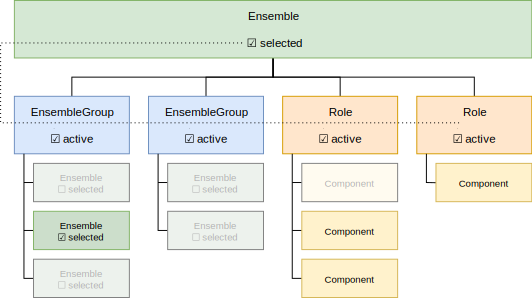
\includegraphics{img/classdia.pdf}
    \caption{Ensemble object diagram}
    \label{fig:objectdiagram}
\end{figure}

One notable feature is that an ensemble does not hold its members directly. Instead, it
holds \cc{MemberGroup}s. Selection parameters in each group are independent from other
groups; that way it is possible to have dynamically selected \cc{ensembles} and
selection enforcement by \cc{rules} in the same ensemble.

Ensembles also keep track of their own selection status. If an ensemble is selected in
its parent group, it can select its own members; more precisely, its groups are allowed
to select their members.

To facilitate this, ensemble has an \cc{isSelectedVar: BoolVar} representing the
selection status. When adding a role or an ensemble group, its \cc{isActiveVar} is set
to equal the parent ensemble's \cc{isSelectedVar}, as indicated on
figure~\ref{fig:objectdiagram} by the dotted line. If an ensemble is selected, all its
groups become active and can select members. If it is not selected, its groups are
inactive and the whole branch of the hierarchy is effectively turned off.

If an ensemble is part of an ensemble group, its \cc{isSelectedVar} is reified with the
corresponding membership constraint in the group's \cc{allMembersVar} (plus the result
of its situation predicate). The root ensemble is not a member of any groups, so its
\cc{isSelectedVar} is bound to true by the policy object.

\section{From Scala to DSL}
\label{impl:scala}

The Scala language has many features which make it suitable as a host language for an
internal DSL. The ability to use blocks of code as expressions allows us to define
custom language constructs. By-name parameters enable delayed evaluation, a necessary
feature for writing declarative code in otherwise mostly imperative language. Arbitrary
nesting, together with code in class bodies, makes the resulting language flow feel
natural. Scala's type system allows us to retain advantages of strong typing and build
generic containers that do the right thing --- and at the same time, type inference is
powerful enough so that users of the DSL almost never come into contact with type
annotations. Finally, operator overloading lets us emulate primitive types with custom
classes, and implicit conversions ensure that the emulated types interoperate with the
built-in ones.

This section describes the overall architecture of the framework, and technical details
of all language constructs used in the DSL. Although we give a brief overview of each
language feature that we are using, this section is mostly intended for readers already
familiar with the Scala language.

%%%

\subsection{DSL Constructs}
\label{impl:scala:verbs}

The DSL uses a number of distinct language constructs. An ensemble definition is, in
Scala terms, implementing a child class:

\begin{lstlisting}[style=snippet]
class MyEnsemble extends Ensemble { /* ... */ }
\end{lstlisting}

Creating a dynamic role is realized as creating a member field from the result of a
function call:

\begin{lstlisting}[style=snippet]
val role = subsetOf(members)
\end{lstlisting}

The call runs directly in the class body. In Scala, this means that it is executed as
part of the constructor.

Scala does have first-class functions, but it does not have \textit{top-level}
functions. Each function must be defined within a class. Functions that are available at
ensemble definition time are in fact methods of the class \cc{Ensemble}. Their results
are tied to the enclosing \cc{Ensemble} instance, which is also where the registration
actually happens; if the result of \cc{subsetOf} in the above snippet was not saved to a
member variable, the selection from \cc{members} would still happen behind the scenes.

This is also one of the reasons ensemble instances must be explicitly registered with
\cc{rules} or \cc{ensembles}: without the registration call, the enclosing instance
would not know about the nested instances. While it would technically be possible to
examine the class through reflection and find all \cc{Ensemble} instances in member
attributes, this would be needlessly fragile in practice.

\medskip

Apart from ``functions'', the DSL also makes use of ``constructs''. The following code
looks distinctly different from the above:

\begin{lstlisting}[style=snippet]
utility {
    val occupied = occupants.size + assignees.cardinality
    occupied * occupied
}
\end{lstlisting}

Although \cc{utility} looks more like a keyword or a flow-control statement, it is in
fact a normal method. Its definition could look like this:

\begin{lstlisting}[style=snippet, language=Scala]
def utility(util: Integer)
\end{lstlisting}

I.e., it is a method that takes a single argument of type \cc{Integer}. The special
syntax is enabled by two useful properties of Scala.

One, code blocks are expressions whose value is the last expression in the block. In
this case, the value of the code block is \dop{occupied * occupied}. Given that a code
block is an expression like any other, it is possible to use code blocks in unusual
places, such as function arguments. The following is a contrived but perfectly valid
example of Scala code:

\begin{lstlisting}[style=ensembles, language=Scala]
val maximum = math.max(
  {
    val a = someFunc()
    if (a > 5) a
    else {
        val b = someOtherFunc()
        a + b
    }
  }, 0)
\end{lstlisting}

Two, Scala allows omitting parentheses in certain conditions. In particular, when
calling a function with one argument, it is possible to omit the enclosing parentheses
if the argument is a code block enclosed in curly braces. The following three statements
are equivalent:

\begin{lstlisting}[style=snippet]
utility(3)
utility({ 3 })
utility { 3 }
\end{lstlisting}

This way it is possible to define methods that can behave as custom language constructs.
Note that this feature is particularly useful in combination with by-name parameters.
See section~\ref{impl:scala:byname} for detailed explanation.


%%%

\subsection{Ensemble Structure}
\label{impl:scala:ensemble}

Each \cc{Ensemble} instance contains the following data:
\begin{itemize}
    \item Collection of role objects, representing dynamically assigned roles
    \item Collection of \cc{EnsembleGroup} objects for each \cc{rules} or \cc{ensembles}
    call
    \item Collection of constraints, in the form of callables that return a \cc{Logical}
    \item Collection of associated security actions and notifications
    \item Situation predicate, if defined
    \item Utility function, if defined
\end{itemize}

For each type of data, methods are available for configuring this data at ensemble
definition time.

As the total number of methods is rather large, and the related functionalities are
mostly independent, each is implemented in a separate trait. We maintain separation of
concerns between traits and declare their dependencies through inheritance and self-type
annotations.

Trait inheritance works the same as normal class inheritance. Most of ensemble traits
inherit from \cc{Initializable}, allowing them to override the \cc{_init} method and
access the solver instance; see section~\ref{impl:scala:initialization} for details.
Inheritance also allows us to inject implicit conversions from \cc{CommonImplicits}
trait.

Self-type annotation in a trait enforces that any concrete class implementing that trait
must also conform to the declared self-type. This usually means that it must implement
some other trait. For example, the following self-type in trait \cc{WithRoles} informs
the compiler of a dependency on two other traits:
\begin{lstlisting}[style=snippet]
trait WithRoles {
  this: WithConstraints with WithSelectionStatus =>
  /* ... */
}
\end{lstlisting}

The \cc{WithRoles} trait is then allowed to access members of the other traits on self.

Functional difference between inheritance and self-type annotation is subtle, but the
takeaway is that self-types define a looser coupling, because they do not lock-in the
inheritance hierarchy. We use self-types to declare that a trait \textit{uses} a
functionality from another trait, but is not an extended version of it.

\medskip

The following list describes the individual traits of \cc{Ensemble}.

\newenvironment{trait}[1]%
    {%
        \par\vspace{0.6em}
        {\bfseries\ttfamily\raggedright\large#1}
        \setlength{\parindent}{0em}
        \setlength{\parskip}{0.3em}
        \begin{adjustwidth}{1cm}{}
    }%
    {%
        \end{adjustwidth}
    }%

\pagebreak

\begin{trait}{Initializable}
    Provides an initialization hook, plus access to the solver instance through the
    \cc{_solverModel} property.
\end{trait}

\begin{trait}{CommonImplicits}
    Defines implicit conversion from \cc{Int} to \cc{Integer}, from \cc{Boolean} to
    \cc{Logical}, and adds methods to collections of \cc{MemberGroup}s. This makes those
    implicit conversions available in ensemble definition context.
\end{trait}

\begin{trait}{WithName}
    Provides a \cc{name} property. Mainly for debugging purposes.
\end{trait}

\begin{trait}{WithActions}
    Provides \cc{allow}, \cc{deny} and \cc{notify} functions, and a method to collect
    results of these functions from sub-ensembles. To achieve that, it has a dependency
    on \cc{WithEnsembleGroups}.
\end{trait}

\begin{trait}{WithConstraints}
    Provides the \cc{constraint} function, storage of registered constraints, and
    functionality related to converting constraints to solver objects.
\end{trait}

\begin{trait}{WithEnsembleGroups}
    Provides the ability to register groups of sub-ensembles, and the \cc{rules} and
    \cc{ensembles} methods. Because groups must activate themselves based on the parent
    ensemble selection status, this trait requires \cc{WithSelectionStatus}.
\end{trait}

\begin{trait}{WithRoles}
    Provides the ability to register roles via role functions. Because roles implicitly
    use constraints, and the \cc{subsetOf} function allows adding a constraint on the
    subset cardinality, this requires the \cc{WithConstraints} trait. In addition,
    \cc{WithSelectionStatus} is required to support group activation based on ensemble
    selection status.
\end{trait}

\begin{trait}{WithSelectionStatus}
    Provides a \cc{BoolVar} indicating the ensemble's selection status.
\end{trait}

\begin{trait}{WithUtility}
    Provides methods to define and query the utility expression of the ensemble, and
    collects utility value from sub-ensembles. To access sub-ensembles, this trait
    requires the \cc{WithEnsembleGroups} trait.
\end{trait}

\medskip

The \cc{Ensemble} class itself defines the \cc{situation} function and handling of the
situation predicate. While it would be straightforward to extract this functionality to
a separate trait, we opted to keep it in \cc{Ensemble}. The functionality is small
enough that it does not clutter the class, esp. given that \cc{Ensemble} is otherwise
empty; and it does not figure in the dependency graph, so extracting it would have
little benefit for the rest of the code (unlike \cc{WithSelectionStatus}, which is also
small and uncomplicated, but is a dependency of two other traits).

%%%

\subsection{Implicit Conversions}

Scala's implicit conversions allow values of one type to be automatically converted to a
different type, if they appear in a context where the target type is required. Two kinds
of implicit conversions are available. With \cc{implicit def}, a function returning the
target type is applied to the value in question. An \cc{implicit class} creates an
instance of a new class, effectively allowing to add new methods to existing types.

Code that uses implicit conversions is less readable, because there are non-local hidden
calls. In the following example, an implicit conversion adds a method named \cc{foo} to
a value of type \cc{Int}. It is impossible to know what is \cc{foo} just from this
snippet; one would need to locate all methods named \cc{foo} in the codebase and then
figure out which implicit conversion is in play.
\begin{lstlisting}[style=snippet]
val x: Int = 7
val y = x.foo()
\end{lstlisting}
\noindent
For this reason, it is usually better to avoid implicit conversions in normal code.
However, they can be extremely helpful when creating a DSL.

For an implicit conversion to take effect, its function or class must be in scope:
either defined in the same class (or a parent class), or explicitly imported.

\medskip

We use implicit conversions for several different purposes. The most common one is
upgrading \cc{Int}s to \cc{Integer}s and \cc{Boolean}s to \cc{Logical}s. This is
important for seamless interoperability of native integer or boolean expressions with
solver constraints, as described in section~\ref{impl:solver:constraints}. The
appropriate conversion functions are defined in trait \cc{CommonImplicits}, which is
mixed in where required. Importantly, it is mixed into the main \cc{Ensemble} class,
thus ensuring that user code will have these conversions in scope whenever defining an
ensemble.

\medskip

Implicit conversions also help cut down on the number of different method overloads. The
method \cc{unionOf} accepts either an iterable of \cc{MemberGroup}s, or a variable
number of \cc{MemberGroup} arguments. However, we want to support using \cc{Component}s
for \cc{unionOf} directly. Otherwise, every time the user wanted to make an union of a
role and a fixed list of components, they would need to specify a role for the component
list. Scala has no support for union types, so it would be impossible to specify a
function that takes a variable number of ``\cc{MemberGroup} or \cc{Component} or
\cc{Iterable[Component]}'' arguments.

Instead, an implicit conversion from \cc{Component} or \cc{Iterable[Component]} to
\cc{MemberGroup[Component]} is defined, allowing the users to use either roles or fixed
sets of components interchangeably.

Similarly, the \cc{allow}, \cc{deny} and \cc{notify} verbs should accept components,
list of components, or roles as their arguments. In the \cc{notify} case, it is simple
enough to provide three overloads for three acceptable argument types. However,
\cc{allow} and \cc{deny} have two arguments of this type. A full set of overloads would
need 9 variants of each verb. Instead, each of these verbs only accepts
\cc{MemberGroup}s as arguments, and implicit conversions ensure that components and
lists of components are usable as well.

\medskip

Two distinct implicit conversions are used with ensemble collections. First, an
\cc{EnsembleGroup} converts to a list of all its members, so that methods like \cc{map}
can be used on results of \cc{rules} call directly. Second, an implicit class
\cc{WithMembersIterable} adds methods \cc{cardinality} and \cc{allDisjoint} to
collections of \cc{MemberGroup}s. This enables the following common idiom:
\begin{lstlisting}[style=snippet]
val r = rules(/* list of ensembles */)
constraint { r.map(_.someRole).allDisjoint }
\end{lstlisting}
\noindent
The variable \cc{r} of type \cc{EnsembleGroup} is converted to \cc{Iterable[E <:
Ensemble]}, so that \cc{map} can be applied on it. This iterable is a plain sequence of
objects of the appropriate ensemble type, which has a member role \cc{someRole}. The
result of the map is therefore a plain sequence of \cc{MemberGroup} objects.

This sequence is then implicitly converted to a class \cc{WithMembersIterable}, which
has the method \cc{allDisjoint}, ensuring that no member is selected more than once for
\cc{someRole}.

Note that the implicit conversion turns the \cc{EnsembleGroup} into a list of
\textit{all} its members, not just the selected ones. This is because at the time the
conversion is used, the list of selected members is not yet known.

The provided methods work due to the fact that inactive (not selected) ensembles do not
have any members. Empty roles add zero to \cc{cardinality}, and are guaranteed to be
disjoint with non-empty ones.

An implicit conversion from an \cc{EnsembleGroup} to its \cc{allMembers} carries some
risk of confusion when used in an inappropriate context. E.g., when inspecting a
solution, the user might inadvertently invoke the implicit conversion and their code
will visit even ensembles that are not part of the solution. We consider this risk
acceptable because, again, ensembles that are not selected do not have any members.

%%%

\subsection{Operator Overloading}
\label{impl:scala:operators}

Method names in Scala are allowed to use special characters, and operators are defined
as regular methods with the appropriate name. For instance, overloading the \dop{+}
operator on an \cc{IntegerInt} type could look like this:
\begin{lstlisting}[style=snippet]
def +(other: Integer): Integer = other match {
    case IntegerInt(value) => new IntegerInt(value + this.value)
    // ...
}
\end{lstlisting}
\noindent
Combined with implicit conversions, both of the following will work:

\begin{lstlisting}[style=snippet]
val leftHand: Integer = someInteger + 5
val rightHand: Integer = 5 + someInteger
\end{lstlisting}
\noindent
The first case is simple. The expression \dop{someInteger + 5} is interpreted as
\dop{someInteger.+(5)}. Because \cc{someInteger} has a \dop{+} operator, Scala tries to
use it. The operator is defined for an \cc{Integer}, and there is an implicit conversion
available that upgrades \cc{5} to \cc{Integer}. The resulting instance is passed to the
\dop{+} method.

The second case is slightly more complicated. As before, the expression translates to
\dop{5.+(someInteger)}. In this case, the built-in \cc{Int} type does not have an
appropriate \dop{+} operator for handling anything \cc{someInteger} could be converted
to. It is necessary to search the list of possible implicit conversions of the left-hand
operand, to see if one of them comes with an appropriate definition of \dop{+}.

\medskip

This process works fine for most operators, but fails for \dop{==}. The problem here is
that \dop{==} is defined on the root class \cc{Any} with the following signature:

\begin{lstlisting}[style=snippet]
final def ==(arg: Any): Boolean
\end{lstlisting}
\noindent
The method is final, so it cannot be overridden. It calls the \cc{equals} method
internally, which is available for overriding, but then the return value is
\cc{Boolean}, which is not appropriate when we need the result as a \cc{Logical}.

It is possible to overload a specialized version of \dop{==} with a different return
type. For the \cc{Integer} trait, the following definitions are desirable:

\begin{lstlisting}[style=snippet]
def ==(other: Integer): Logical
def ==(other: Int): Logical
\end{lstlisting}
\noindent
We need to have a special variant for \cc{Int}, because implicit conversion won't help
us here: \dop{someInteger.==(5)} can use the default implementation for type \cc{Int}.

The problem with this is that the integration is not seamless. If the \cc{Int} value
appears on the right-hand side, it will always be able to use the built-in \dop{==}.
This is made worse by the fact that both of the following will compile:

\begin{lstlisting}[style=snippet]
val l1: Logical = someInteger == 5
val l2: Logical = 5 == someInteger
\end{lstlisting}
\noindent
The type of \dop{5 == someInteger} is \cc{Boolean}, which has an implicit conversion to
\cc{Logical}, and so it is valid in every context that requires a \cc{Logical} type. But
the result of the comparison is always false, because we are comparing unequal types.

\medskip

The \cc{Integer} trait uses a triple-equals \dop{===} operator for comparing equality in
the desired way. This is a convention used by many other Scala-based DSLs and language
customizations. Scala compiler will emit a warning whenever two unrelated types are
compared with \dop{==}, which should notify the user that they made a mistake.

We considered raising an exception in an overridden \cc{equals} method, but that would
silence this warning, and would not work when \cc{Int} is the left-hand operand anyway.

%%%

\subsection{Type Bounds}

One of the features required from the DSL is seamless working with different ensemble
and component types. Consider the following code:
\begin{lstlisting}[style=ensembles]
class Worker(val rank: String) extends Component
val workers: Iterable[Worker] = /* ... */
class Root extends Ensemble {
    val supervisor = oneOf(workers)
    constraint { supervisor.all(_.rank == "supervisor") }
    allow(supervisor, "supervise", workers)
}
\end{lstlisting}

The \dop{supervisor.all()} call must accept a function whose argument is of type
\cc{Worker} --- otherwise, it would be impossible to access the \cc{rank} attribute.
That means that \cc{supervisor} must carry the information that its member type is
\cc{Worker}, not just a generic \cc{Component}. At the same time, the \cc{allow} call
must accept \cc{supervisor} as its argument.

\pagebreak
Roles are of type \cc{MemberGroup}, which is generic over its member type. The signature
looks like this:
\begin{lstlisting}[style=snippet]
class MemberGroup[+MemberType]
\end{lstlisting}

The \dop{+} symbol indicates that the class is \textit{covariant} in the \cc{MemberType}
argument. That means that for superclass \cc{A} and its subclass \cc{B},
\cc{MemberType[B]} is considered a subclass of \cc{MemberType[A]}.

Method \cc{MemberGroup.all} accepts functions of type \cc{MemberType => Boolean}. In our
example, member type is \cc{Worker}.

Method \cc{accept} takes an argument of type \cc{MemberGroup[Component]}, so it accepts
a \cc{MemberGroup[Worker]} object.

The type signature of \cc{oneOf} looks like this:
\begin{lstlisting}[style=snippet]
def oneOf[C <: Component](items: Iterable[C]): MemberGroup[C]
\end{lstlisting}
The method takes an iterable of objects of concrete type \cc{C}, which is a subtype of
\cc{Component}, as indicated by the \dop{<:} symbol. It returns a \cc{MemberGroup}
parameterized by the appropriate concrete type. Scala's type inference makes sure that
when passing an iterable of \cc{Worker}s, the returned \cc{MemberGroup} will have
\cc{Worker} as its member type.

\medskip

Ensemble groups work in a similar way, except that \cc{EnsembleGroup} is a subclass of
\cc{MemberGroup} specialized so that its member type must be a subtype of \cc{Ensemble}.
This is the signature:
\begin{lstlisting}[style=snippet]
class EnsembleGroup[+EnsembleType <: Ensemble]
    extends MemberGroup[EnsembleType]
\end{lstlisting}

The \dop{+} symbol indicates type covariance: an \cc{EnsembleGroup} of a concrete
type of ensemble is a subclass of \cc{EnsembleGroup[Ensemble]}. The \dop{<:} symbol
indicates a type bound: the member type must be a subtype of \cc{Ensemble}.

Similar to role functions, \cc{rules} and \cc{ensembles} must be defined with
appropriate type signatures, so that they return the appropriate variant of
\cc{EnsembleGroup}.

%%%

\subsection{Initialization}
\label{impl:scala:initialization}

Every ensemble and group object requires an instance of the solver, through which
variables and constraints are constructed. This is not available at ensemble definition
time.

In terms of Scala, the whole policy is a series of instances of nested classes. In order
to propagate a solver object, the user of the DSL would be required to add parameters to
their ensemble class definitions and manually propagate them when instantiating
sub-ensembles. This violates separation of concerns: the solver object is an
implementation detail of the framework, not something the users should care or even know
about.

Instead, the ensemble tree is constructed without access to the solver, and the solver
object is passed to it in a separate initialization step. The \cc{Initializable} trait
defines a method \cc{_init}, which allows classes and traits to hook into the
initialization process. The \cc{Policy} object calls \cc{_init} on the root ensemble,
and the \cc{Ensemble} class is responsible for propagating the call to its ensemble
groups and role objects. Ensemble groups are in turn responsible for propagating the
call to sub-ensembles. This way it is ensured that every part of the policy tree is
initialized.

The initialization runs in three phases:
\begin{enumerate}
  \item \cc{ConfigPropagation} propagates a \cc{Config} object, which contains the newly
  created instance of the solver.
  \item \cc{VarsCreation} is the phase where solver variable objects are created. The
  class \cc{MemberGroup} initializes its set and activation variables, and \cc{Ensemble}
  initializes its selection variable.
  \item \cc{RulesCreation} can use variables created in the previous step to generate
  and post solver constraints.
\end{enumerate}

While it might be possible to perform the initialization in a single pass, it would make
it more difficult to implement properly. Developers would need to be extra careful about
initialization order, e.g., make sure that an initialization step is not using variables
from a child (or parent) object whose initialization isn't finished yet. Multi-phase
initialization removes this source of fragility. Phase (1) can be done by every object
individually. Phase (2) only requires that the solver is available, i.e., that phase (1)
has finished everywhere, and phase (3) can rely on the fact that \textit{all} variables
across all objects have been generated in the previous phase.

\medskip

Several component traits of \cc{Ensemble} implement their own \cc{_init} steps. This is
possible because Scala has a well-defined trait linearization order, and calling
\cc{super._init()} within a trait will invoke the \cc{_init} implementation in the next
trait up.

%%%

\subsection{By-Name Parameters}
\label{impl:scala:byname}

As stated in section~\ref{impl:scala:initialization}, the solver object is not available
at ensemble definition time --- or, more precisely, at ensemble instantiation time. Most
of constraint definition and role creation is done in class body, and this code actually
runs when the corresponding instance is constructed. This poses two related but distinct
problems.

First, consider a role that relies on external data:

\begin{lstlisting}[style=ensembles]
class Scenario(val workers: mutable.ArrayBuffer[Worker]) {
  class Root extends Ensemble {
    val role = subsetOf(workers)
    constraint { role.cardinality > 5 }
  }
  val policy = Policy.root(new Root)
}

object Scenario {
  def main() {
    val scenario = new Scenario(/* ... */)
    scenario.policy.resolve()
    scenario.workers.append(new Worker(/* ... */))
    scenario.policy.resolve()
  }
}
\end{lstlisting}

One would expect the second \cc{resolve} call to use the newly added \cc{Worker}
instance. However, at that point, the ensemble seems to already exist, and the old value
of \cc{workers} was used to construct \cc{role}. Groups register their members at
construction time (see section~\ref{impl:solver:groups}), so the original argument no
longer affects the set of role members.

It would be useful if the framework could somehow ``refresh'' the policy definition
using new data.

Second, the \cc{constraint} statement works with \cc{role.cardinality}. We expect the
result to be a \cc{Logical} object referencing an underlying \cc{BoolVar}. But as stated
above, at this point the solver instance is not available, so a \cc{BoolVar} cannot be
created.

Both of those issues are solved using \textit{by-name parameters}.

\medskip

In Scala, functions are first-class objects, so naturally it is possible to pass them as
arguments explicitly. That is what happens in this statement:
\begin{lstlisting}[style=snippet]
val role = subsetOf(members, _ > 1)
\end{lstlisting}
The expression \dop{_ > 1} is a shortcut for \dop{x => x > 1}. This is a function of
type \dop{Integer => Logical}, i.e., takes an \cc{Integer} argument and returns a
\cc{Logical}.

By-name parameters are basically parameters that are passed as functions implicitly. The
signature of a \cc{constraint} verb is:
\begin{lstlisting}[style=snippet, language=Scala]
def constraint(clause: => Logical): Unit
\end{lstlisting}
\cc{clause} is a by-name parameter, and its type is ``expression of type \cc{Logical}''.
The important point is that unlike normal parameters, the expression is not evaluated
until actually used in the \cc{constraint} method body. Furthermore, the following
works:
\begin{lstlisting}[style=snippet]
val clauseFun: () => Logical = clause _
\end{lstlisting}
Using the above syntax, the ``expression'' parameter is converted to a normal function
with no arguments. The \cc{constraint} method stores all such functions in a collection
and only runs them in the \cc{RulesCreation} initialization phase, when the solver is
available and all variables are already created.

The verbs \cc{situation} and \cc{utility} also take by-name parameters and call them
at appropriate times.

\medskip

Section~\ref{dsl:c:root} specifies that the root ensemble must be instantiated in the
\cc{Policy.root} method. The reason is that the argument of this method is actually a
by-name parameter too. The policy object does not store the instantiated policy tree, it
stores a \textit{builder} function which constructs it. On every call to \cc{init()} or
\cc{resolve()}, the policy tree is instantiated from scratch, and so it reflects the
current values of all external variables.

%%%

\subsection{Variadic arguments}

Many functions that accept iterables also accept variadic arguments. For example, it is
possible to call \cc{oneOf} in two ways:
\begin{lstlisting}[style=snippet]
val a = oneOf(listOfMembers)
val b = oneOf(memberA, memberB, memberC)
\end{lstlisting}

Scala natively supports variadic arguments. For the following two signatures, the type
of \cc{items} is the same:
\begin{lstlisting}[style=snippet, language=Scala]
def oneOf(items: Seq[Component])
def oneOf(items: Component*)
\end{lstlisting}

One minor issue with the second signature is that it allows the list of arguments to be
empty. This does not cause any problems in practice --- after all, the user could as
well pass an empty list of components --- but still, it would be cleaner to disallow
code like \dop{val x = oneOf()}.

To achieve this, all variadic functions actually have two arguments: one is mandatory,
the other is variadic. This is the definition of \cc{oneOf}:
\begin{lstlisting}[style=ensembles, language=Scala]
def oneOf[C <: Component](itemFirst: C, itemRest: C*): Role[C] =
    oneOf(itemFirst +: itemRest)
\end{lstlisting}
Type of \cc{itemFirst} is \cc{C}, and type of \cc{itemRest} is \cc{Seq[C]}. The code
prepends the first item to the list and calls the other overload of \cc{oneOf}. It is
possible to call \cc{oneOf} with one or more arguments; calling with no arguments is
illegal.


\chapter{Evaluation}
\label{evaluation}

To evaluate practicality and performance characteristics of our approach, we have
designed a number of testing scenarios. Each tests a particular aspect or feature of the
DSL.

\section{Methodology}

In this chapter, we take \textit{scenario} to mean a particular situation or task with
possible variables. A \textit{configuration} is an instance of the scenario, where the
variables are bound to particular values. A \textit{test case} is a set of
configurations to be evaluated. In a test case, each configuration is usually tested
many times, and each attempt is called a \textit{test run}.

E.g., a scenario can be described as: ``pick several Workers and one Leader from a pool
of Persons''. A configuration of that scenario can be ``pick one Worker and one Leader
from a pool of 15 Persons''. One test case involving this scenario can be a set of
configurations ``pick three Workers and one Leader from a pool of $N$ Persons'', with $N
\leftarrow 10, 15, 20... 100$. Another test case would be ``pick $N$ Workers and one
Leader from a pool of 100 Persons'', with $N \leftarrow 1, 2... 20$

Each scenario is represented by a class containing the necessary objects and a
definition of the associated ensemble(s). A companion \cc{Spec} subclass is a concise
description of scenario parameters and an interface for the test runner. It generates
appropriate instances of the scenario class on which each test run is performed.

Because Scala runs in a Java Virtual Machine (JVM) with Just-in-Time compilation, it is
necessary to ``warm up'' for the given scenario. Otherwise, earlier test runs would be
slower than the later ones, where the JIT has had time to catch up and pre-compile hot
paths. To prevent this, the smallest configuration is run repeatedly for 10 seconds of
wall-clock time.

We run each configuration a specified number of times and record the time to find a
solution, utility (if specified), and peak memory usage for each run. Raw data from the
results can be found in the accompanying archive in \texttt{results} directory,
organized by test case name. Graphs are generated with Python, using
scipy~\citep{scipy}, pandas~\citep{pandas}, and matplotlib~\citep{matplotlib}. It is
possible to regenerate them by executing the script \cc{python/all.sh}.

All results are generated on an Intel\textregistered{} Core\texttrademark{} i5-6600K
CPU, running on a single core at 3.90 GHz.

\subsection{Time Limits}

In most scenarios, we set a solver time limit to 30 seconds per test run. This number
was chosen as an arbitrary cut-off point. Preliminary experiments showed that observed
trends are robust even below 30 seconds, and increasing the time limit has diminishing
returns in terms of solution quality (see also section~\ref{eval:example:limits}).
Setting a higher time limit would significantly prolong test times while providing very
little additional useful data.

Moreover, 30 seconds seem like a reasonable real-world time limit. The framework is
designed for highly dynamic scenarios and needs to be able to respond to changing
conditions as they happen. Waiting more than a couple seconds for access control
decisions is not acceptable in terms of user experience, and could possibly even
endanger the security goals of the system. Taken in this context, even 30 seconds is
possibly too long. Our results show that in real-world scenarios it might be possible to
lower the time limit further.

\subsection{Memory Usage}

The JVM provides a memory-managed environment with asynchronous garbage collection,
which makes it difficult to obtain reliable memory usage information. As a rough
measure, our test runner uses garbage collector notifications from the Java Management
Extensions API~\citep{jmx} to record peak memory usage during each test run. We trigger a
GC cycle between test runs, and attempt to wait until the cycle is complete. This is
inherently unreliable, however, and there is no way to ensure that all unreachable
objects have been released.

As measured with this method, most scenarios use less than 200 MB of memory. These
results cannot be used to draw any conclusions: any trends are lost in the variance,
allocator granularity, and general overhead of the JVM runtime.

In section~\ref{eval:variables}, we test relatively large configurations where memory
consumption is significant. Although the data about memory usage is still very noisy, it
provides some useful insights. We note that the measured data does not reflect true
memory requirements; many scenarios can run with much less memory available, by doing
garbage collection as needed during the computation.

We have configured the JVM to use a maximum of 10 GB of RAM for its heap. This ensures
that our chosen test configurations never need to deal with memory pressure, which
considerably reduces timing jitter.

%%%%%

\section{Basic Benchmarks}
\label{eval:variables}

To evaluate performance of the basic building blocks, we have designed a scenario that
selects one of a list of 100 000 members. With the \cc{oneOf} function, there is already
a constraint specifying that the cardinality of the selection is 1. From there, we
generate large numbers of additional meaningless constraints. Given that finding a valid
solution is trivial, results of this test provide information about per-constraint
processing time and memory consumption.

\medskip

To evaluate simple constraints, we generate a number of \cc{constraint} statements
specifying that selection cardinality must be smaller than $i$ for an increasing $i$. In
the constraints test case, the total number of constraints $N$ goes from 50~000 to
1~000~000.

\medskip

To evaluate \cc{Logical} expressions, we generate the following expression:
\begin{lstlisting}[style=snippet]
val condition: LogicalBoolVar = role.cardinality === 1
condition && condition && condition && /* ... repeated N times */
\end{lstlisting}
\cc{condition} creates a single \cc{BoolVar} in the solver, and the repeated use of the
\dop{&&} operator constructs an unbalanced tree of \cc{LogOp} operations of a specified
length. In this test case, $N$ goes from 500 to 10~000.

\medskip

To evaluate \cc{Integer} expressions, we generate \cc{IntVar}s by repeating idempotent
arithmetic operations. As explained in section~\ref{impl:solver:arithm}, every
arithmetic operation creates a new \cc{IntVar}. As the starting value, we use the
selection cardinality, and repeatedly add 15 to it and then subtract 15 from it $N$
times. Finally, we post a constraint that the selection cardinality must be equal to the
new value, so that the solver is forced to propagate the results of all the individual
calculations. In this test case, $N$ also goes from 500 to 10~000.

Every configuration of every test case runs 100 times.

\medskip

Figure~\ref{fig:variables:time} shows timing results. Each point represents median time
to solve a configuration of a given size. Standard deviation across runs was under
150~ms in most cases, so we choose not to display it in the graph.

\begin{figure}[t]
    \centering
    \includegraphics[width=1\linewidth]{img/variables.pdf}
    \caption{Computation times for basic building blocks}
    \label{fig:variables:time}
\end{figure}

Computation time for constraints grows linearly with the total number of constraints,
and 750~000 constraints can be processed in about 5 seconds. This would match the
intuition that the solver needs to evaluate each constraint once to ensure that the
tested solution is valid.

An interesting point is the discontinuity around the 750~000 mark. This is most likely
caused by the corresponding discontinuity in memory usage, as discussed below.

Computation time for integers also grows linearly, which matches the intuition that the
sequence of arithmetic operations must be propagated in linear time. The results also
closely follow the time measured for simple constraints. Each point represents two
arithmetic operations per element, so we can conclude that each arithmetic operation
takes roughly as much processing time as 50 simple constraints.

Computation time for logical operations grows quadratically and runs out of the allotted
30-second time limit at 8~000 operations. A \cc{Logical} operation does not create new
variables in the solver, and the full expression is posted as a single constraint. The
quadratic behavior comes from an inefficiency in Choco's CNF normalization, which does
not deal well with the unbalanced expression we are submitting. Still, 4~000 logical
operations can be done under 5 seconds.

\medskip

Figure~\ref{fig:variables:mem} shows peak memory usages. Each point represents a maximum
over the configuration runs. Memory usage data has an extremely high variance, sometimes
on the order of hundreds of megabytes, which we chalk up to the unreliability of our
measurements. Nevertheless, the maxima paint a clear picture.

\begin{figure}[t]
    \centering
    \includegraphics[width=1\linewidth]{img/variablemem.pdf}
    \caption{Memory consumption for basic building blocks}
    \label{fig:variables:mem}
\end{figure}

Memory usage for constraints grows linearly, but shows a distinct discontinuity between
400~000 and 700~000 elements. As noted above, this corresponds to a discontinuity in
processing time. We do not have an explanation for this behavior. However, the
discontinuity starts before memory usage reaches 4~GB and returns to original projection
at around 8~GB. We therefore hypothesize that this could be an artifact of JVM memory
allocator behavior, or perhaps a custom allocator in Choco.

Memory usage for integers also grows linearly, in a much more predictable manner. We
note that in this test case, the recorded peak usage resembles the actual usage more
closely than in other tests. In previous experiments, when only 4 GB were allocated to
the JVM, the integer test case ran out of memory at around 7~500 elements, and
computation time started to rise sharply around the 4~500 mark --- presumably due to
memory pressure and the need to run GC during the computation. The other test cases did
not run into similar problems; GC runs were causing timing jitter, but other than that,
the constraint test case continued linearly until 950~000 elements, and the logical
operation test case was unaffected.

The logical operation test case reaches a plateau at the 1~500 mark, rising only very
slowly in subsequent configurations. We expect that this corresponds to some
pre-allocated internal array whose size is sufficient for all our configurations; given
that the first jump is from 2 GB to 4 GB, it is possible that at some larger
configuration the pre-allocated array would grow twice as large again. The \cc{LogOp}
tree and associated data is very small in comparison.

\section{Evaluating the Running Example}
\label{eval:example}

The security policy from the running example contains both static and dynamic elements,
and showcases all major features of the framework. It is therefore a good starting point
for evaluation. We have designed a number of testing scenarios based on it.

To quickly summarize, the security policy manages a building with workrooms, which are
statically assigned to projects, and lunchrooms, which are unassigned and limited by
capacity. At lunch time, workers can request seats in lunchrooms and the policy should
grant them access as soon as a seat becomes available, while upholding the overall
security goal: workers from different projects must not use the same room.

There are two main types of sub-ensembles in the policy. \cc{WorkroomAssignment} is
registered for each project and allows workers of the project to enter all workrooms
of that project. \cc{LunchroomAssignment} is registered for each lunchroom and ensures
that seats in that lunchroom are allocated as appropriate.

%%%

\subsection{Static Assignments}

The first scenario is in the morning, when workrooms are already open, but lunchrooms
are closed. Per the situation predicate, \cc{LunchroomAssignment}s are inactive, so only
statically-assigning \cc{WorkroomAssignment}s will be in play. Measuring their behavior
should give us a performance baseline.

There are 100 workrooms that are assigned in a round-robin fashion to the configured
number of projects. We have set up three test cases, for 5, 15, and 50 projects. In each
case, we vary the number of workers from 500 to 10~000 in increments of 500. Each
configuration is tested 500 times.

\begin{figure}[ht]
    \centering
    \includegraphics[width=1\linewidth]{img/workers-simple.pdf}
    \caption{Static assignment to workrooms}
    \label{fig:workers-simple}
\end{figure}

Figure~\ref{fig:workers-simple} shows the results of measurements. Vertical lines from
the points represent error bars of one standard deviation; in many cases, too small to
be visible over the point marker.

Computation time grows linearly with the total number of access grants. For this reason,
times for the 5-project test case are larger: the number of workrooms is fixed, so each
project gets more rooms and each worker gets an access grant to each of the rooms.

The measurements are in the millisecond range, and it is possible to process 10~000
workers in 80~ms. Most of the time is actually spent pre-generating a lookup table for
the \cc{allows()} method; when this feature is disabled, computation times drop as much
as 4x for the largest configuration.

%%%

\subsection{Empty Lunchrooms}
\label{eval:example:dynamic}

At lunch time, \cc{LunchroomAssignment} ensembles are activated, and workers can request
seats by setting their \cc{hungry} attribute to true. In the second scenario, we assume
that all available lunchrooms are empty, and the solver is attempting to seat an
increasing number of hungry workers.

From the outset, it is clear that the problem has an exponentially large solution space.
The solver is attempting to maximize a utility expression: $\sum |s_i|^2$, where $s_i$
is the set of occupied seats in $i$-th lunchroom. Even with the knowledge that only the
cardinality of seatings matters, the search still needs to implicitly consider all
possible assignments of projects to lunchrooms, and all possible distributions of
workers between the available rooms.

\begin{figure}[ht]
    \centering
    \includegraphics[width=1\linewidth]{img/workers-morerooms.pdf}
    \caption{Dynamic assignment with more rooms than projects}
    \label{fig:workers-morerooms}
\end{figure}

The test case in figure~\ref{fig:workers-morerooms} has 4 lunchrooms with 10 seats
each, and 3 available projects. Individual configurations then specify a total number
of hungry workers, which are selected from the projects in a round-robin fashion.

The Y axis represents time to find an optimal solution. Each configuration is rendered
as a box plot over the test runs, with whiskers representing 1.5 IQR, and outliers
removed. The blue line is an exponential curve fitted to the medians.

Even in this very small test case, computation times are unacceptably slow. Seating 12
workers takes 5 seconds, and the solver crosses the 30 second time limit at the 16
worker mark\footnote{The solver was able to find the optimal solution under 30 seconds
in several cases, but it timed out in most of the 100 test runs. For this reason, we
have excluded this data entirely.}.

\medskip

The situation with more available lunchrooms than projects represents the worst case for
the solver: it is certain that at least one project will be able to use more than one
room, so workers from that project can be distributed among the available rooms.

This factor is removed in the next scenario. Number of lunchrooms is fixed to 3, each
with 5 seats, and number of projects varies from 5 to 9. Same as in previous scenario,
the lunchrooms are empty and we are seating an increasing number of hungry workers.

\begin{figure}[ht]
    \centering
    \includegraphics[width=1\linewidth]{img/workers-moreprojects.pdf}
    \caption{Dynamic assignment with more projects than rooms}
    \label{fig:workers-moreprojects}
\end{figure}

The search is simplified by the fact that in terms of utility, distributing workers from
the same project across rooms is always worse than putting them together and using
workers from a different project for the other rooms. Although the number of solutions
is still exponential, computation times are much lower.

Figure~\ref{fig:workers-moreprojects} shows the results. Variance in computation times
is comparable to the previous scenario, so we are only showing median times to optimal
solution. Two outlier configurations have been omitted: 6 projects with 35 workers, and
8 projects with 39 workers. See section~\ref{eval:example:badsolver} for discussion.
After that, the longest time recorded is approx. 9 seconds, for 27 workers in 9
projects.

An interesting property is visible here. The peak times correspond to multiples of the
number of projects, and after $4p + 1$ workers, computation times sharply drop to
\textasciitilde{}10~ms. This point corresponds to the moment when the round-robin
algorithm first picks 5 hungry workers (same as lunchroom capacity) from the same
project. As soon as a lunchroom can be filled to capacity by a single project, the
solver seems to be able to use this fact to optimize the search.

Similarly, multiples of number of projects are the points when the same number of
workers is picked from every project. At that point, all projects are equally good
candidates for seating, and so the number of solutions rises; after the peak, it is
possible to quickly exclude the projects with fewer hungry workers.

Although the computation is still relatively slow, we are now within realistic problem
sizes. In a real-world deployment, seating 30 workers in 5 seconds might be acceptable.

%%%

\subsection{Probabilistic Search Anomalies}
\label{eval:example:badsolver}

In the previous scenario, we observed that when a trivial solution of a certain type
exists, the solver converges on that solution very quickly. In particular, when it is
possible to fill a room to capacity, an optimal solution is found in milliseconds. This
result was stable across runs and not affected by the number of ``overflow'' workers who
are hungry but could not be seated.

However, in some cases, the optimization seems to fail. This often appears in the form
of outliers --- in a particular configuration, most attempts take 20~ms, but some can
take several seconds. For some configurations, the short times are actually the
outliers: most attempts take several seconds, and the occasional ``good try'' completes
immediately.

We have not found a pattern in the bad configurations. The outliers in good
configurations behave probabilistically and appear more frequently as configuration size
grows.

To measure this behavior, we have set up the following scenario: the number of projects
is the same as the number of lunchrooms, each lunchroom has a capacity of 5, and there
are 5 hungry workers per project. The trivial solution is apparent: each lunchroom
is filled to capacity with workers from one project, and the remaining search space
is only as big as the number of project-lunchroom permutations.

\begin{figure}[ht]
    \centering
    \includegraphics[width=1\linewidth]{img/badsolver.pdf}
    \caption{Frequency of search anomalies}
    \label{fig:badsolver}
\end{figure}

We created configurations of 1 to 30 projects, and ran 500 tests of each, with a time
limit of 3 seconds. The expected solving time of one run is below 100~ms, so this time
limit was deemed sufficient. Results are shown as a percentile graph in
figure~\ref{fig:badsolver}. We arbitrarily chose to plot multiples of 4. Showing more
configurations does not bring any additional insights and makes the graph less clear.

For 4 projects, all tests finished under 500~ms. At 12 projects, 60~\% of tests finished
under 500~ms, and 25~\% of tests timed out. 28 projects is large enough that no test
finished under 500~ms, but the curve still has a similar shape; presumably, the
likelihood of finding the good solution is too low.

The configuration with 20 projects is a ``bad'' one, as all of the 500 attempts have
timed out.

%%%

\subsection{Solver Time Limits}
\label{eval:example:limits}

In all previous scenarios, we measured time to find an \textit{optimal} solution. When
the search timed out before declaring a solution optimal, it was counted as a failure.
However, that does not mean that \textit{no} solutions were found.

Choco's optimization process works by finding a satisfying solution for the problem and
then posting an additional constraint that the next solution must have a strictly higher
utility. Most of the time this means iterating over several successively better
solutions. If an optimal solution is not required, it is possible to either switch the
behavior of the solver, or to accept the best solution found when the time limit is
reached.

To test the trade-off between speed and solution quality, a scenario was set up with 3
projects, 5 lunchrooms with 20 seats each, and 21 hungry workers, 7 per project. In
this scenario, the optimal solution is seating all of the workers from a single project
in one of the available lunchrooms, and keeping two rooms empty. The total utility
of this solution is $7^2 \cdot 3 + 0 \cdot 2 = 147$.

\begin{figure}[ht]
    \centering
    \includegraphics[width=1\linewidth]{img/timelimits.pdf}
    \caption{Utility of solutions found before time limit}
    \label{fig:timelimits}
\end{figure}

We created configurations with a successively higher time limit from 1 to 30 seconds,
and measured them over 100 runs. Figure~\ref{fig:timelimits} shows each configuration as
a box plot over successful tests, with whiskers representing 1.5 IQR, and outliers
removed. A relatively large amount of tests have failed to find a solution within the
time limit. The red dashed line shows the amount for each configuration. Over 50
attempts were successful in every case, which gives us a sufficient number of samples.

The data has high variance, but the successful runs copy a logarithmic curve (shown in
blue). That is the expected behavior. On an exponential problem, linear increase in
computation time should provide logarithmic benefits.

None of the test runs get close to the optimal utility of 147. In preliminary
experiments, even tests with a time limit of 5 minutes did not converge on the optimal
solution. These results also retroactively show that our choice of 30 seconds as the
default time limit was reasonable.

%%%

\subsection{Practical Situations}
\label{eval:example:practical}

Previous scenarios were testing the solver on arbitrary configurations in isolation. In
a real-world deployment, however, the situation would look very different.

First thing to note is that in practice, it is almost impossible for dozens of workers
to request lunch at exactly the same time. We have experimented with a ``one-by-one''
solving method, where instead of submitting all hungry workers to the solver at once, we
incrementally submit one worker at a time. This converts the $O(k^N)$ problem of seating
$N$ workers to $N$ separate $O(1)$ problems of seating one worker. In most cases, this
approach will achieve the same utility, because workers from the same project are
preferentially seated together. Computation time grows linearly with the number of
workers.

\begin{figure}[ht]
    \centering
    \includegraphics[width=1\linewidth]{img/workers-oneworker.pdf}
    \caption{Time to seating one worker}
    \label{fig:workers-oneworker}
\end{figure}

Figure~\ref{fig:workers-oneworker} shows computation times for seating one worker in an
increasing number of lunchrooms. Each case was measured 100 times. Blue dots represent
median times, vertical lines are error bars of one standard deviation.

The number of projects is irrelevant, as the worker being seated can only belong to one,
and lunchrooms are only tied to projects through their occupants. Lunchroom capacity is
also irrelevant, as long as it is 1 or more. At 200 lunchrooms, one worker can be seated
in one second, which is probably good enough for any reasonable real-world deployment.

Solving time is perfectly quadratic (shown in orange) in the number of lunchrooms. The
source of the quadratic behavior is most likely the \cc{allDisjoint} constraint: a
worker can be seated in any of the $N$ rooms, and for each variant, $N$ rooms must be
checked to ensure disjointness.

%%%

\subsection{Simulation}
\label{eval:example:simulation}

In practical situations, it is also very rare for all lunchrooms to be empty at the
same time. When the first worker is seated in a lunchroom, the choice locks the
worker's project to that room. All subsequent requesters from the same project will be
preferentially seated there. This effectively splits the problem in two: workers from a
chosen project will only be seated to that project's rooms, while these are excluded
from the possibilities for workers of other projects.

In order to examine this behavior, and to test the solver in more real-world-like
conditions, we have created a simulation of worker behavior at lunch time. The basis of
the simulation is a building with 500 workers working on 10 projects, which is realistic
for a modern office building. On each of the 5 floors there is a lunchroom with 40
seats.

At every step of the simulation, every worker that hasn't eaten yet has a 0,5~\% chance
of becoming hungry and requesting a seat. Once a worker receives a seating notification,
they take up to 5 simulation steps to reach the lunchroom, and then 5 to 20 steps to
eat, before leaving the lunchroom and getting back to work.

In a typical simulation run, all workers can have lunch in about 2~000 steps. We are not
particularly interested in the tail end of the simulation, because it mostly involves
waiting for workers to finish eating. Therefore, we stop the simulation after 1~500
steps, and run the first 1~500 steps 100 times, for a total of 150~000 steps.

\begin{figure}[ht]
    \centering
    \includegraphics[width=1\linewidth]{img/simulation.pdf}
    \caption{Histogram of computation times per simulation step}
    \label{fig:simulation}
\end{figure}

Figure~\ref{fig:simulation} is a histogram of computation times per one simulation step,
with both axes logarithmic. The median step time is 6.4~ms, and mean step time is
10.7~ms. Out of the 150~000 measurements, only 285 took more than 100~ms.

There is a small number of outliers that do not find the optimal solution within the 30
second time limit. However, an important feature of this kind of setup is that it can
recover very fast from such failure. In the rare case where a difficult configuration
arises, such as when two lunchrooms become available in the same simulation step, a
sub-optimal seating solution will still place some workers in at least one of the rooms.
Subsequent solver runs can continue off this result and place the remaining workers. We
have never observed more than one failure in a row.

From these results, we conclude that the performance of the framework is suitable for
real-world deployment.



\chapter{Conclusion}
\label{conclusion}

In this work we have presented an ensemble-based approach to defining access control
policies. Security situations are specified in terms of ensembles and their roles, and
access control decisions are attached to the ensembles. This allows the policy to follow
the evolution of a dynamic system as its shape and composition changes over time.

We introduced a framework, TCOOF-Trust, which consists of two parts: a~policy
specification language, implemented as an internal DSL in Scala, and a runtime
environment for resolving the policies. The DSL can be used to specify ensembles, roles,
constraints on their membership, and attached security decisions. The runtime
environment processes the policy specification in the DSL, converts the problem to an
input for its internal CSP solver, and uses the results to determine ensemble
membership. Based on the solution and the rules attached to it, the framework can
respond to access control queries.

We have designed and specified detailed semantics for the behavior of the framework, and
extended the existing TCOOF-Trust prototype implementation to properly support them. A
clean API for embedding the framework in external projects is provided, and detailed
documentation was created for the CSP conversion process and for the implementation
details of the framework.

An example security scenario with dynamic access control requirements was used to
evaluate performance of the framework, both in synthetic and real-world-like
configurations. While the underlying problem is exponential by nature, results show that
the framework is capable of dealing with the complexity in a reasonable manner, and
scales well in practical deployments.


%%% Bibliography
\include{bibliography}

%%% Attachments to the master thesis, if any. Each attachment must be
%%% referred to at least once from the text of the thesis. Attachments
%%% are numbered.
%%%
%%% The printed version should preferably contain attachments, which can be
%%% read (additional tables and charts, supplementary text, examples of
%%% program output, etc.). The electronic version is more suited for attachments
%%% which will likely be used in an electronic form rather than read (program
%%% source code, data files, interactive charts, etc.). Electronic attachments
%%% should be uploaded to SIS and optionally also included in the thesis on a~CD/DVD.
%%% Allowed file formats are specified in provision of the rector no. 72/2017.
\appendix
\chapter{Data Archive Contents}

The data archive accompanying this work is a copy of the \cc{tcoof-trust} GitHub
repository. Its up-to-date version can always be found at the following URL:
\href{https://github.com/matejcik/tcoof-trust}{\ttfamily https://github.com/matejcik/tcoof-trust}

The only additional content in the archive is the \cc{apidoc} directory, which contains
the generated Scaladoc API documentation. In a Git checkout, the API docs can be
generated with the command \dop{sbt doc}.

The following is a list of paths in the archive and descriptions of their contents.

\bigskip

\newenvironment{filepath}%
    {%
        \par\vspace{0.6em}\ttfamily\raggedright
    }%
    {%
        \vspace{-0.2em}
    }%

\begin{filepath}
README.md
\end{filepath}
\begin{dsldesc}
    Markdown-formatted \cc{README} for the Git repository. Please refer to this file for
    requirements to run the TCOOF-Trust framework and basic usage examples.
\end{dsldesc}

\begin{filepath}
build.sbt\\
project/
\end{filepath}
\begin{dsldesc}
    SBT (Scala Build Tool) build script and build properties. These files are required
    for building the project with \cc{sbt}, and for importing into IntelliJ IDEA, the
    preferred Scala IDE.
\end{dsldesc}

\begin{filepath}
apidoc/
\end{filepath}
\begin{dsldesc}
    Scaladoc API documentation in HTML format.

    The limitation of the generated API documentation is that it excludes non-public
    members. Unfortunately, that cannot be avoided with the Scaladoc tool. See the
    source code for documentation comments.
\end{dsldesc}

\begin{filepath}
python/all.sh
\end{filepath}
\begin{dsldesc}
    Shell script that installs the Python environment and regenerates graphs used in
    this work. Must be executed in the \cc{python} subdirectory.
\end{dsldesc}

\begin{filepath}
python/Pipfile\\
python/Pipfile.lock
\end{filepath}
\begin{dsldesc}
    \cc{pipenv} configuration files. Contain list of Python package dependencies
    required for generating graphs.
\end{dsldesc}

\begin{filepath}
python/lunch.py\\
python/other.py\\
python/resultlib.py\\
python/variables.py
\end{filepath}
\begin{dsldesc}
    Individual Python scripts that generate the graphs. \cc{variables.py} generate
    graphs from section~\ref{eval:variables}, \cc{other.py} generates the simulation
    histogram and the timeout graph, \cc{lunch.py} generates all the rest.
    \cc{resultlib} is a small library of common functions.
\end{dsldesc}

\begin{filepath}
results/final/badsolver-growingprojects.log
\end{filepath}
\begin{dsldesc}
    Source data for figure~\ref{fig:badsolver}.
\end{dsldesc}

\pagebreak
\begin{filepath}
results/final/booleans.log\\
results/final/constraints.log\\
results/final/integers.log
\end{filepath}
\begin{dsldesc}
    Source data for figures \ref{fig:variables:time} and \ref{fig:variables:mem}
\end{dsldesc}

\begin{filepath}
results/final/moreprojects.log
\end{filepath}
\begin{dsldesc}
    Source data for figure~\ref{fig:workers-moreprojects}.
\end{dsldesc}

\begin{filepath}
results/final/morerooms-optimizing.log
\end{filepath}
\begin{dsldesc}
    Source data for figure~\ref{fig:workers-morerooms}.
\end{dsldesc}

\begin{filepath}
results/final/oneworker-params.log
\end{filepath}
\begin{dsldesc}
    Source data for figure~\ref{fig:workers-oneworker}.
\end{dsldesc}

\begin{filepath}
results/final/simulated.log
\end{filepath}
\begin{dsldesc}
    Source data for figure~\ref{fig:simulation}.
\end{dsldesc}

\begin{filepath}
results/final/timelimits.log
\end{filepath}
\begin{dsldesc}
    Source data for figure~\ref{fig:timelimits}.
\end{dsldesc}

\begin{filepath}
results/final/workercount-simple.log
\end{filepath}
\begin{dsldesc}
    Source data for figure~\ref{fig:workers-simple}.
\end{dsldesc}

\begin{filepath}
src/main/scala/cz/
\end{filepath}
\begin{dsldesc}
    Scala source files for the TCOOF-Trust framework, specifically the package
    \cc{cz.cuni.mff.d3s.trust}.
\end{dsldesc}

\begin{filepath}
src/main/scala/scenario/
\end{filepath}
\begin{dsldesc}
    Scala source files for the test measurement scenarios.
\end{dsldesc}

\begin{filepath}
src/test/scala/
\end{filepath}
\begin{dsldesc}
    Scala source files for the unit test suite.
\end{dsldesc}

\begin{filepath}
thesis/
\end{filepath}
\begin{dsldesc}
    \LaTeX{} source files and a PDF version of this work.
\end{dsldesc}
    

\openright
\end{document}
